\section{Experiment 1: Reducing training data with care}

% Corresponding Progress Reports
% https://www.notion.so/241122-Matthias-first-exploration-for-image-dropout-ccb558156ba04efab6435b0f42021d44
% https://www.notion.so/241129-Matthias-Dropout-experiment-first-results-dac4111347ec413c87bbdfdaf4ef495e?pvs=23
% https://www.notion.so/241213-Matthias-iCNN-in-image-dropout-9e810b27443c400f902e232cf966004d?pvs=23
% https://www.notion.so/241220-Matthias-reducing-train-data-with-care-First-AI-captions-0a0a3c610dba4d9c84d4eda4fb1c53dd?pvs=23
% https://www.notion.so/20250117-Matthias-Filling-the-gaps-1-7126a49b2ee34921aff7e853c3a1542c?pvs=23
% https://www.notion.so/Matthias-Mildenberger-243a8aff9cee491a987bc227e5c937cc?p=ef08526d469548adbeedae4384177db1&pm=s
% https://www.notion.so/250214-matthias-filling-the-gaps-4-197726ec52d680a28b00db7958f00613?pvs=23

\subsection{Background}

\rTwo{
As established earlier, the diversity of training data may play a crucial role in determining the performance of brain activity reconstruction. In this first experiment we investigate how different aspects of data diversity ranging from low-level features (such as colors and shapes) to high-level features (such as semantic concepts) influence the image reconstruction from brain activity. Since increasing the data diversity by recording new data is very resource-intensive (recording new data takes time and money), we take a backward approach: we reduce the training data in a strategic way. The reduction will be performed under different subsampling criteria, which relate to different aspects of data diversity (ranging from low-level to high-level features). The aim is to find a way to reduce the training data that allows a reconstruction performance similar to (or even better than) the full data set. This will allow a first exploration of what aspects should be considered when creating a possible new training data set with maximized diversity, that could achieve the best possible results in future new experiments where new brain activity can also be recorded.}

Many studies have explored how to achieve comparable results with reduced training data sets as with the full data set. Wang et al.~\cite{wangDataDropoutOptimizing2018} used a two-step procedure, first training the model on the full training data and then using the validation data to delete any training samples that would reduce the overall loss on the validation data set. This allowed them to remove unfavourable training samples and to end up training a new model on a reduced dataset, which actually performed better than the full dataset. Sener et al.~\cite{senerActiveLearningConvolutional2018} were able to use a core set approach in active learning to ensure that the data selected during model training would yield the greatest improvement, thus achieving good classification even with greatly reduced datasets. They were able to outperform many other algorithms and a random subselection baseline. In a detailed review, Guo et al.~\cite{guoDeepCoreComprehensiveLibrary2022} compared different approaches to core set selection, highlighting in particular that random subselection is still a very strong baseline, often outperforming many sophisticated core set approaches. In a dataset for medical imaging of the heart, Kolluru et al.~\cite{kolluruLearningFewerImages2021} were able to reduce the data to almost a tenth of its original size and still achieve acceptable results. They first used an autoencoder to map the images into an abstract feature space, then used PCA to further reduce the dimensionality, and finally used the k-medoids algorithm to form as many clusters in the reduced space as there were images to be extracted from the dataset. In summary, guided reduction of training data is a promising approach to achieving stable performance with significantly fewer resources during training (and presumably data collection).

\rTwo{Various approaches can be used to create subsamples based on maximising the diversity of different features. To create subsamples that maximize the diversity of low-level features (colours, shapes, textures) simple approaches for example based on the distribution of colours in an image~\cite{maheshwariImageClusteringUsing2009} could be used. More sophisticated approaches that can also cover mid-level and high-level features of images may use the activation of pre-trained deep learning models to embed images in a more abstract feature space. In this space semantic clustering becomes possible~\cite{chang2017deep}. Birdokar et al.~\cite{birodkarSemanticRedundanciesImageClassification2019} use different feature layers of a CNN to perform image clustering at different levels (low, mid and high level features). The late layer was especially useful for extracting the semantic features of the images and clustering was used to remove redundant samples. To make clustering algorithms such as k-means computationally feasible, the data from the extracted features should be reduced in dimensionality fist. UMAP~\cite{mcinnesUMAPUniformManifold2018} is a modern nonlinear dimensionality reduction algorithm. In order to cluster the images in a low-level space, UMAP can also be applied directly to the images without first embedding them in a feature space. After the dimensionality reduction, the subsampled datasets can be generated by using clustering such as k-means.}

With respect to \rOne{translating} brain activity, it has been previously found that different levels of the visual system are also better at predicting different feature levels (i.e., low-level brain structures such as V1 and V2 are better at predicting low-level features, and high-level structures such as PPA and FFA are better at predicting high-level features)~\cite{horikawaGenericDecodingSeen2017}. However, to the best of our knowledge, there has been no systematic investigation of how maximising the diversity of training data at different feature levels (low-level vs.\ high-level) affects the \rOne{translation} of brain data and the subsequent reconstruction of images. In other words, whether it is more important to have a training set that contains as many different semantic concepts as possible, or to use a training set that contains as many different low-level features (e.g.\ colours and shapes) as possible. 

\rTwo{Building on these considerations, we hypothesize that the feature level at which training data diversity is maximised will directly influence reconstruction performance on test data. Specifically, we expect that the \rOne{translation} and reconstruction of artificial shapes will benefit most from emphasizing low-level feature diversity, as these images are predominantly defined by basic visual attributes such as shape and color. Conversely, reconstruction performance on natural images should improve when prioritizing high-level diversity, since accurate predictions depend on capturing semantic concepts. Additionally, we hypothesize that a balanced, mid-level approach that integrates both low-level and high-level diversity will yield the best overall performance across both image categories. To test the effectiveness of these diversity-based strategies, we include random subselections of the training data as baselines.}


\subsection{Methods}

The procedure for obtaining a reduced training data set with maximised diversity is described below.

\subsubsection{Baseline with random dropout}

\rTwo{In order to evaluate the diversity-based methods, it is important to establish a suitable baseline against which the results can be compared. To this end, reconstruction will first performed on a randomly subsampled training set. To get a better idea of the size of the training set needed to train the \rOne{translators}, different data fractions will be used. The full training set consists of 1200 images (and the corresponding recorded MRI activity). For the baseline, 10\% (120 images), 25\% (300 images), 50\% (600 images), 75\% (900 images) and 100\% of the images will first be used to train the \rOne{translator}. This baseline investigation will only be performed for one subject (S2) to save computational resources. To control the sampling error, 5 random samples will be taken for each data fraction and used to train the \rOne{translators}. If all training images are used, only one sample can be taken (the full data set). The results of this random baseline investigation will then be used to determine the sample size needed for the diversity based dropout.}


\subsubsection{Diversity based data subsampling}

For this work, the data should be subsampled as diversely as possible in order to produce a reduced dataset that can beat a randomly subsampled dataset in terms of \rOne{translation} and reconstruction performance. In this work, a multi-step subsampling procedure is chosen: First, all training images are transformed into a latent feature space. Within this feature space, an attempt is made to maximise diversity. Then, the nonlinear dimension reduction algorithm UMAP~\cite{mcinnesUMAPUniformManifold2018} is used to reduce the dimensionality of the training images' embeddedings in the respective feature space to two dimensions. The data in the UMAP space is then divided into $k$ clusters using k-means clustering (where $k$ is the number of images to be subsampled). For each of the $k$ clusters, the centroid of all $n$ images in that cluster is determined. Finally, for each cluster, the image with the smallest Euclidean distance to the centroid is selected. Using this procedure, $k$ images can be subsampled, where $k$ is arbitrary but must be less than the total number of training images. However, it should be clear that $k$ clusters cannot reasonably be found in the selected feature space; for example, if $k$ is selected very high (about 50\% of the dataset), only 2 images would be present in each cluster. To ensure that the subsampling algorithm can produce a meaningful subselection of the training set, k should be chosen as small as possible. Given the results of the random subselection baseline in the previous chapter, $k$ is set to 25\% (i.e. 300) of the images in the training set. 

% 4 UMAP
\begin{figure}[ht]
    \centering
    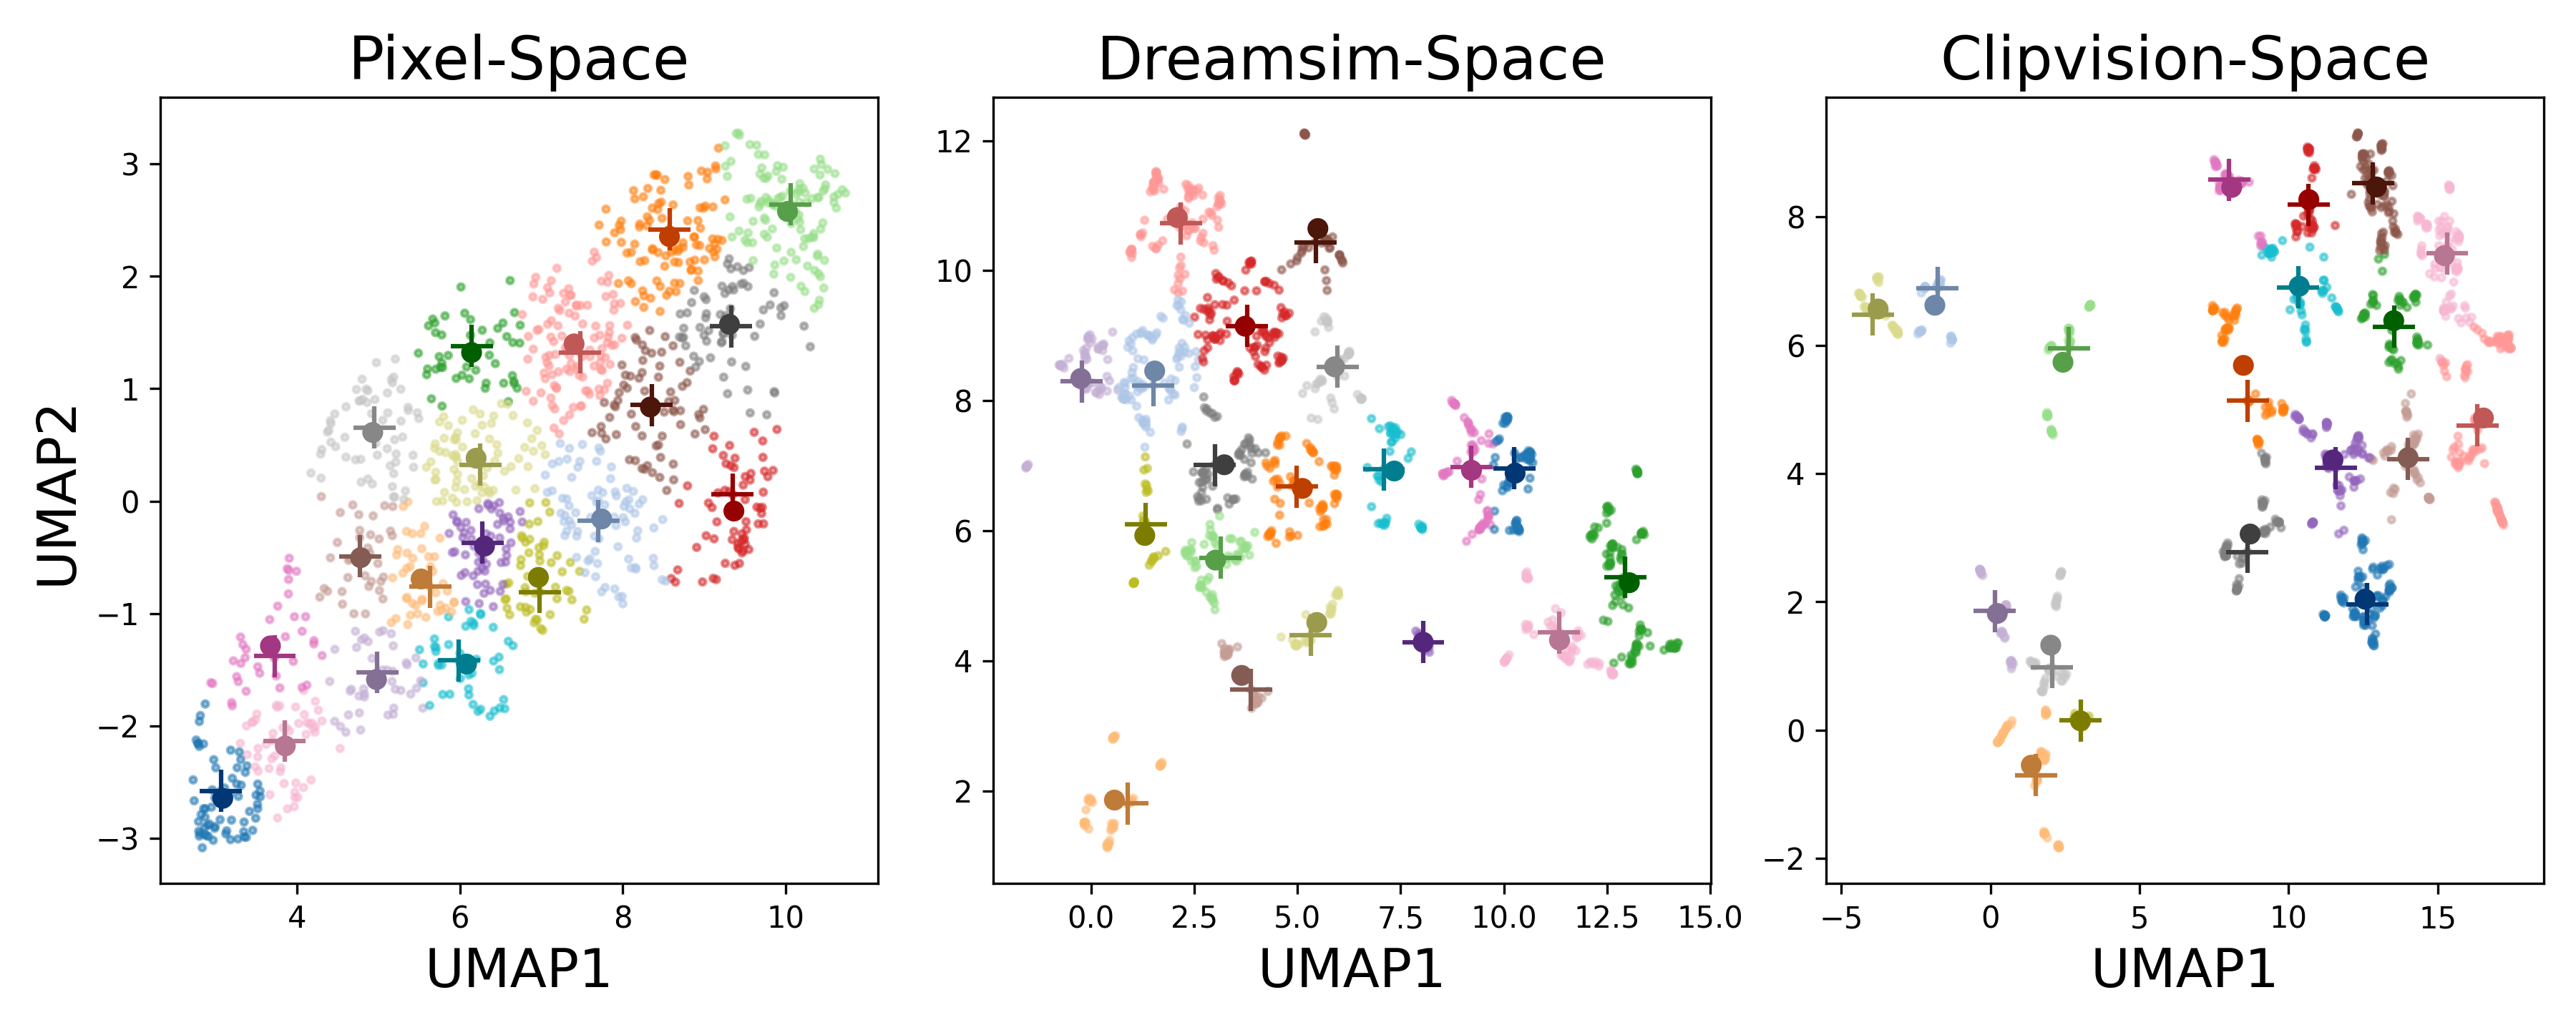
\includegraphics[width=0.9\textwidth]{plots/dropout_umap.png}
    \caption[UMAP visualization of diversity based subsampling]{Visualization of the two dimensional UMAP embeddings of the Pixel-Space, the dreamsim-space and the CLIP Vision space. Each point stands for one image in the training dataset. The x and y axis depict the dimensions that the UMAP algorithm computes. The points are colorized using k-means clustering (each cluster gets a different color). The mean value of all images in a cluster is visualized with a cross and the image that is closest to this mean value is visualized as a thick circle.}\label{fig:dropout_umap}
\end{figure}


The feature space in which the training images are initially embedded is freely selectable. To follow the logic of the evaluation criteria, a low-level, a mid-level and a high-level representation are chosen. For the low-level representation, the images (resized to 200$\times$200 pixels) are simply concatenated into a one-dimensional vector, so that the subsequent UMAP algorithm reduces the dimensions at the pixel level (this procedure was successfully applied by the authors of UMAP to the MNIST dataset). For the mid-level representation, the training images are embedded with dreamsim~\cite{fuDreamSimLearningNew2023}, for the high-level representation, the training images are embedded in CLIP-space using CLIP Vision~\cite{radfordLearningTransferableVisual2021}. Thus, all images are transformed into one-dimensional vectors whose dimensionality is reduced subsequently using UMAP and is then clustered using k-means. 
An example of the results of the selection process is shown in Figure~\ref{fig:dropout_umap}. In the plots, the number of clusters has been set to $k=20$ for visualisation purposes. Each point in the plot represents a sample of the training data set in UMAP space. Each cluster is coloured differently. The centroid of each cluster is shown as a circle and the image closest to the centroid is marked with a cross. In dreamsim and CLIP Vision space, the different clusters are already clearly separated from each other in the two dimensions of UMAP, while the result in pixel space has divided the images comparatively homogeneously, which may indicate that the UMAP dimension reduction has not worked optimally (this can probably be explained by the high number of dimensions in pixel space 200$\times$200$\times$3 colour channels = 120000). 

In order to ensure that the created subselection indeed increases the diversity in the feature space, it is validated quantitatively. For this purpose, a new metric is defined, the average minimum distance to all training samples (Average Min Distance). It is defined as follows:

\[
\text{Average Min Distance}
\coloneq \frac{1}{n_{\text{all}}}
  \sum_{i=1}^{n_{\text{all}}}
    \min_{1 \le j \le n_{\text{sub}}}
      \Bigl\lVert f(z_i) - f(z_j) \Bigr\rVert
\]\myComment{Changed images from x to z}

\noindent{}\rTwo{where \( n_{\text{all}} \) represents the number of images in the full dataset, \( n_{\text{sub}} \) represents the number of images in the subsample, \( z_i \) represents the $i$-th image in the full dataset, \( z_j \) represents the $j$-th image in the subsample, \( f \) represents embedding function from image to feature space and \( \|\cdot\| \) represents the Euclidean (L2) norm.}

The Average Min Distance measures how close on average each image in the full training dataset (embedded in the respective feature space) is to the closest image in the subsample. If the subsample adequately represents the feature space, then for each input image there would be a comparatively close candidate in the subsample. 

\subsection{Results}

\rTwo{The results of the random subsampling will be analyzed to determine a proper sample size for the diversity based dropout. Then the created diversity based subsamples will be analyzed. Finally, the the three diversity based subssamples and the random subsample will used to train the \rOne{translator} and reconstruct images for each of the five subjects.}


\subsubsection{Random dropout}
The performance of the \rOne{translator} is shown in Figure~\ref{fig:dropout_random_translator} for both the natural test images and the artificial shapes. For the natural test images, the relationship between the number of training samples and performance is relatively similar for all the \rOne{translators}: the more training samples, the better. However, for the VDVAE and iCNN in particular, the performance curve for the \rOne{translator} flattens out at around 50\% training samples. The trend for the artificial shapes is somewhat different. The CLIP Vision \rOne{translator} does not seem to improve with an increasing number of training images, but is only just above the random level of 0.5. The \rTwo{CLIP Text} \rOne{translator} can show a performance above the random level from about 50\% of the training data set and then increases continuously. The VDVAE \rOne{translator} shows a slightly higher performance, but also saturates at about 50\% of the training data set. The same pattern is shown by the iCNN, whose performance is the best, but also does not improve after about 50\% of the training data set. 

\begin{figure}[ht]
  \centering
  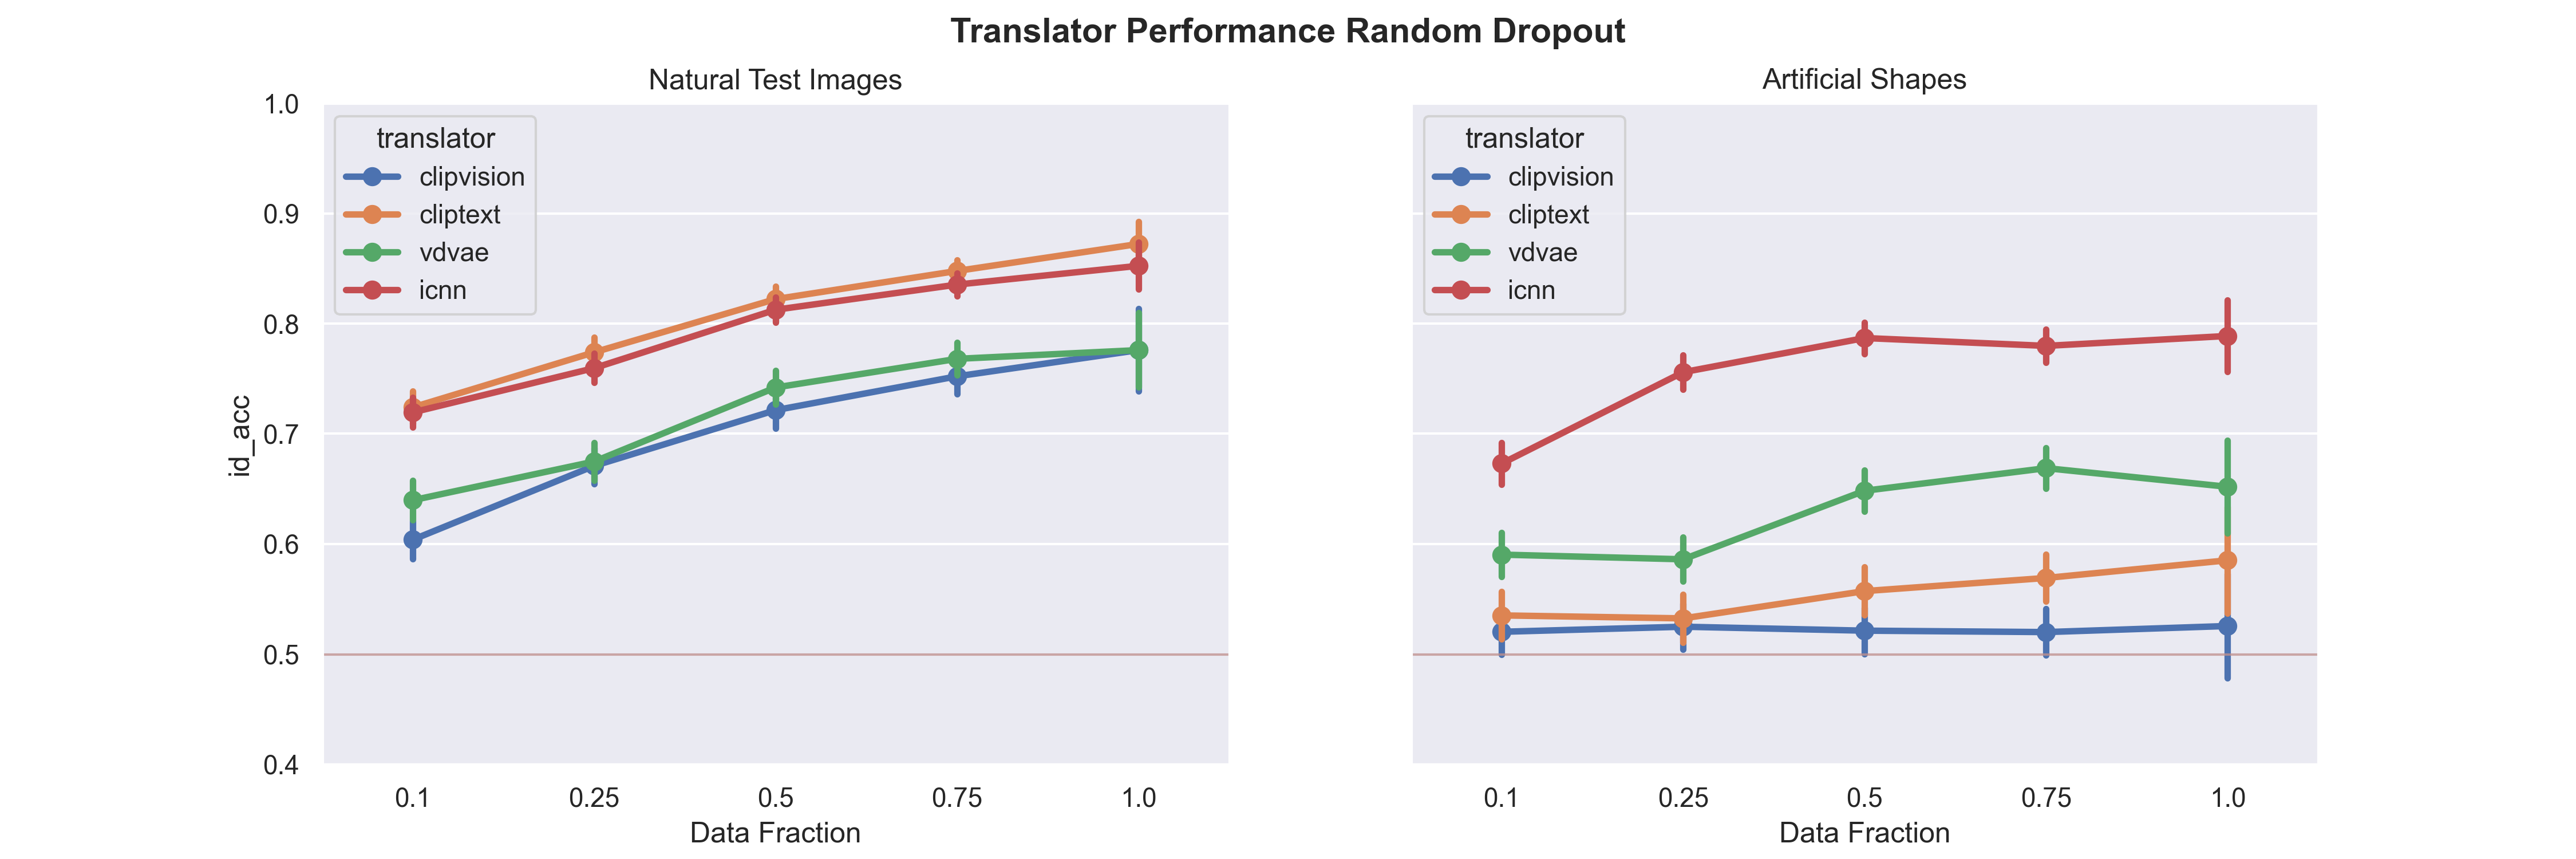
\includegraphics[width=1\textwidth]{plots/dropout_random_translator.png}
  \caption[Translator Performance with increasing dropout]{\rOne{Translator} Performance with different levels of random dropout \rOne{for subject S2. The four different translators were trained with random samples of the training dataset at different sizes (from 10\% to 75\% of the original size) and the performance is displayed using the identification accuracy. For each subsampled size, five random samples were drawn, the errorbars are computed as the standard error across the five subsamples.}}\label{fig:dropout_random_translator}
\end{figure}

The quantitative performance of the reconstruction algorithms is shown in Figure~\ref{fig:dropout_random_reconstruction} for both the natural test images and the artificial images. The PixelCorrelation shows a similar picture for both algorithms for the natural test images and the artificial shapes: While the iCNN benefits from more training samples, with the step from 25\% to 50\% of the training data set being particularly significant, the Brain-Diffuser shows only a very small increase in performance with increasing number of training samples. The dreamsim similarity increases continuously with a larger number of training samples. In particular, the iCNN benefits from a larger number of training samples. The CLIP-accuracy shows that for the natural test images the performance also saturates at about 50\% of the training samples, the same goes for the artificial shapes.

\begin{figure}[ht]
  \centering
  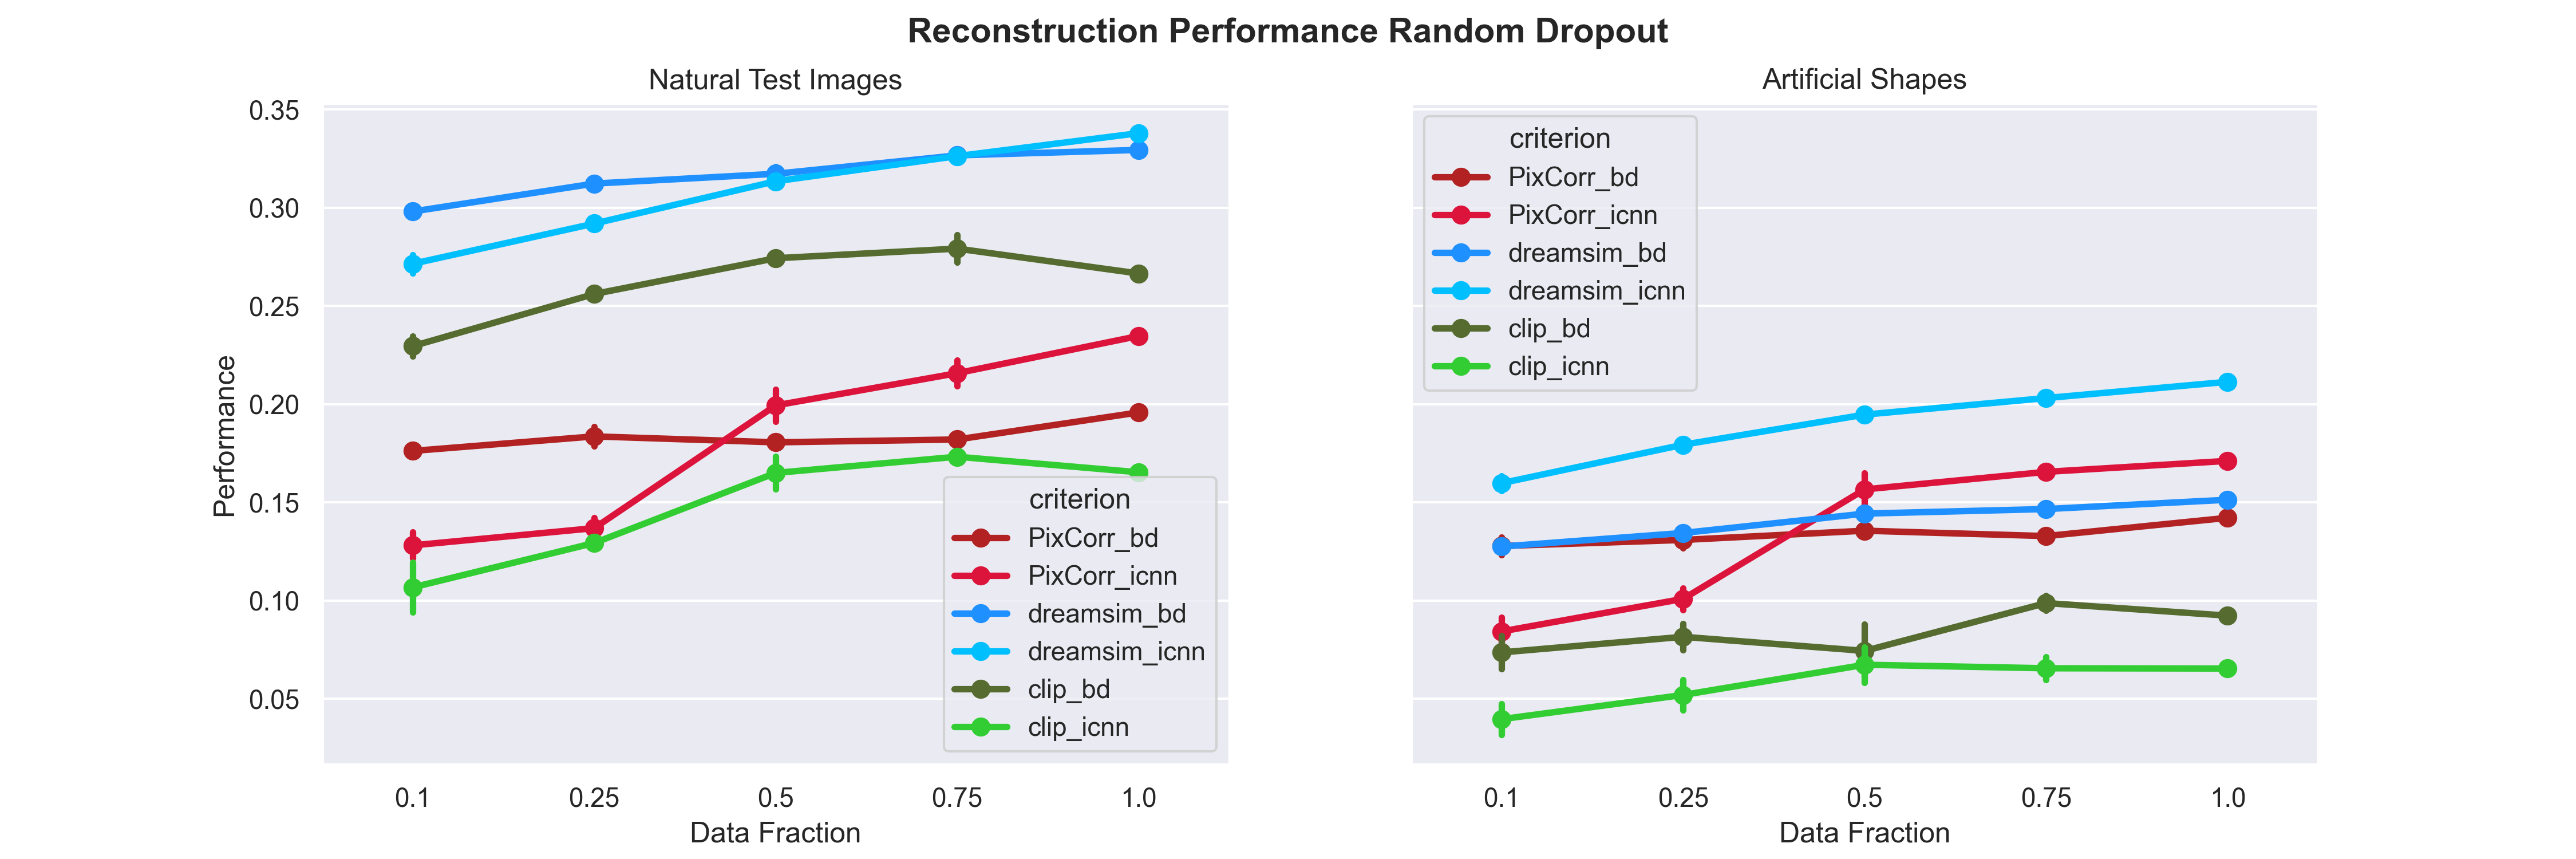
\includegraphics[width=1\textwidth]{plots/dropout_random_reconstruction.png}
  \caption[Reconstruction Performance with increasing dropout]{Reconstruction performance with different levels of random dropout for subject S2. The translators for the reconstruction algorithms were trained with random samples of the training dataset at different sizes (from 10\% to 75\% of the original size). The performance is displayed using the three reconstruction criteria PixelCorrelation, dreamsim and CLIP-accuracy. For each subsampled size, five random samples were drawn, the errorbars are computed as the standard error across the five subsamples.}\label{fig:dropout_random_reconstruction}
\end{figure}

The qualitative performance of the reconstructions with different training set sizes can be seen in Figure~\ref{fig:dropout_qual_random_test} for the natural test images. It can be seen that even with only 10\% of the training images, distinctive features of the images can be reconstructed, \rTwo{while it's also visible, that} the quality of the reconstructions improves as the amount of training data increases. For example, the Brain-Diffuser is not yet able to correctly classify the snowmobile as a vehicle with a small amount of training data, or the outlines of the goldfish are not yet nearly correct with the iCNN.\@ Interestingly, the reconstruction of the Brain-Diffuser's aircraft is better with a small number of training samples than with the full data set. This is probably because the VDVAE, which produced artefacts for this image, still works with the small number of training samples. \rTwo{For the artificial shapes a very similar picture emerges, the quality of reconstructions improves visibly with an increased number of training samples. An example of their reconstruction for the random dropout can be seen in the appendix in figure~\ref{fig:dropout_qual_random_art}.}


\begin{figure}[H]
  \centering
  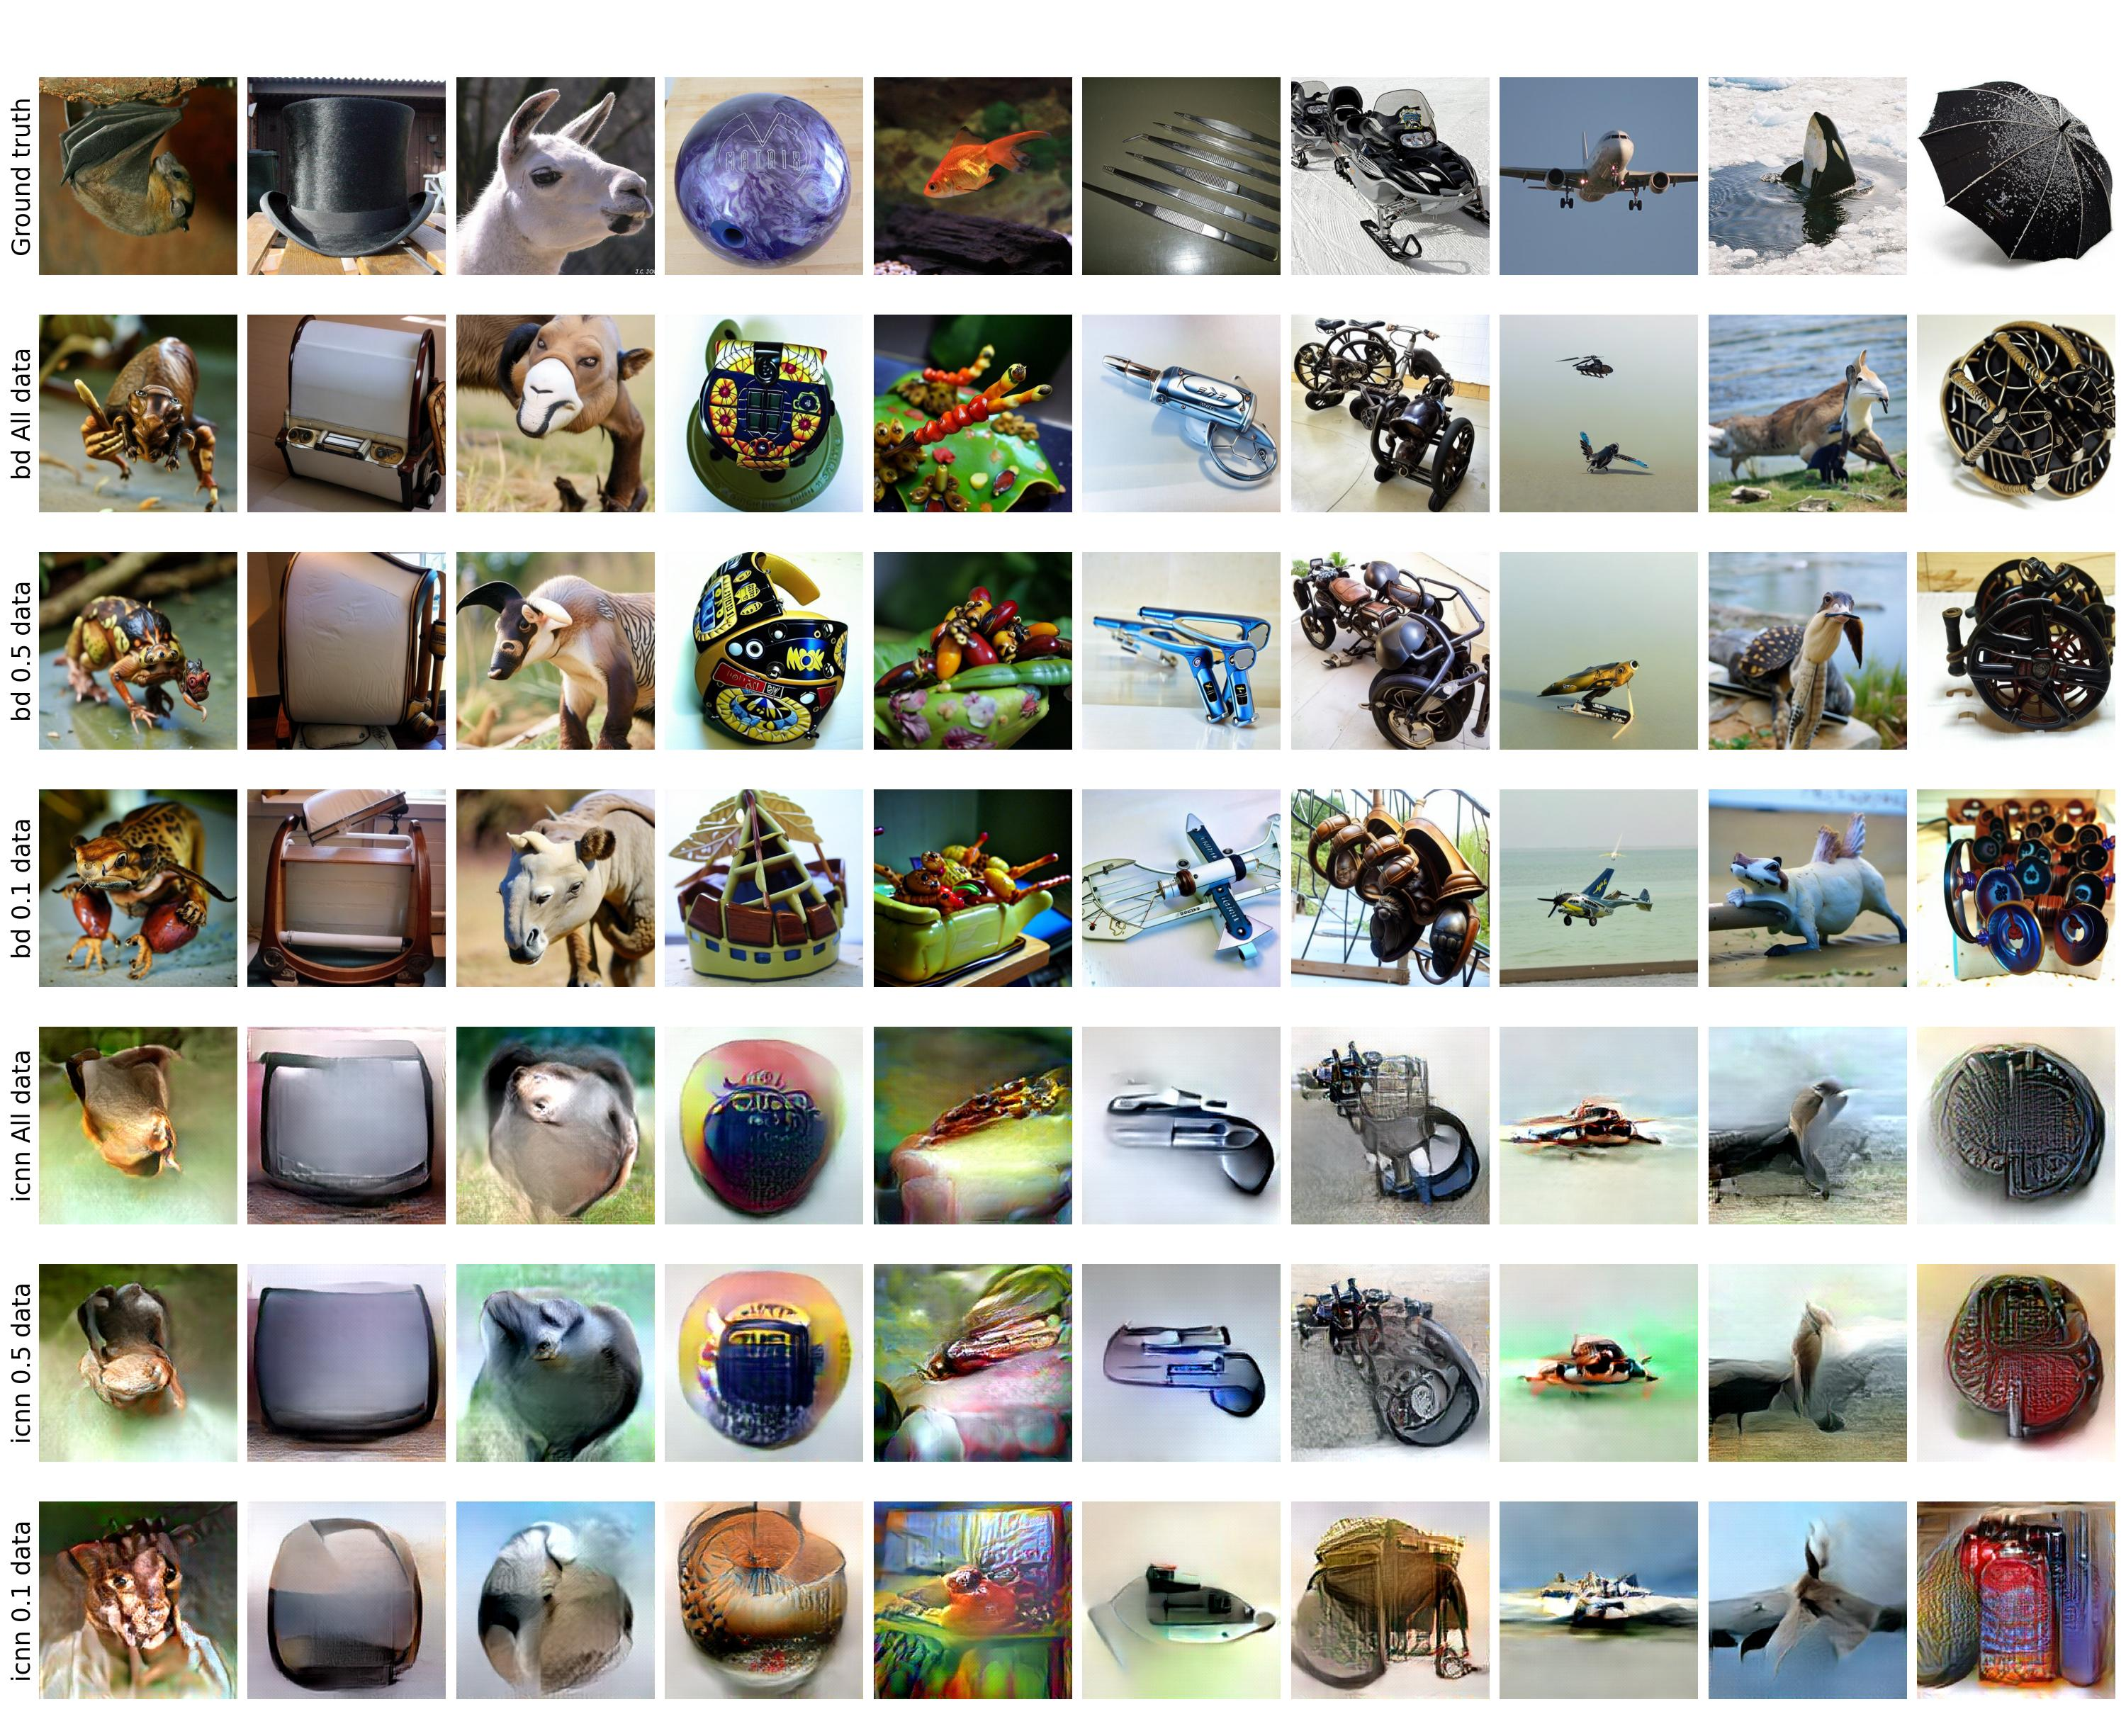
\includegraphics[width=1\textwidth]{plots/dropout_qual_random_test.JPEG}
  \caption[Qualitative results random dropout on natural test images]{Qualitative results with different levels of random dropout on natural test images. In the first row, the ground truth images are displayed. In the following three rows, the reconstructed images from the Brain-Diffuser are displayed with three different sizes of the training data (either all data, a 50\% random subsample of the data and a 10\% random subsample of the data). In the last three rows, the reconstruction results from the iCNN are displayed, again with the three different training dataset sizes.}\label{fig:dropout_qual_random_test}
\end{figure}

In summary, it can be said that the performance in \rOne{translation} and reconstruction can usually be significantly improved with an increasing number of training samples. In our example, many effects become visible in the step between 25\% and 50\% of the training data set, and in some cases the performance starts to saturate from this point on. For the following experiments, therefore, the data set should not contain more than 50\% of the training samples, in order to still have potential for performance improvement. At the same time, the training data set should not be smaller than 25\%, otherwise the \rOne{translation} may not work well enough for testing.


\subsubsection{Diversity based dropout}
\rTwo{According to the previously described procedure to gain diversity based subsamples,} subsamples with 25\% (300 images) of the training data set were extracted for each of the feature spaces using the method described above. Figure~\ref{fig:dropout_similarity_plot} shows an example of five training dataset images (left column), where the most similar image in the subsampled dataset in the respective feature space is displayed. This shows the differences in sampling in the three feature spaces: in the dreamsim and CLIP Vision spaces, the images are relatively similar to the original. \rTwo{There are also small} differences between the mid-level and high-level similarities that become clear. For example, in the case of the revolver in the first image, dreamsim selects a gun that is relatively similar in the image, but is the wrong type. CLIP Vision selects an image that is a better semantic match because it also shows a revolver, even though the remaining visual similarity is lower (colour of the gun, partially covered by a hand). This difference between CLIP Vision and dreamsim can also be seen in other images. In pixel space the subjective similarity between the original and the sample is lower and based on the low-level features of the input images disregarding semantic similarities. In the third image, for example, the original shows an ear with white headphones, while the most similar image in pixel space is a goose with a long white neck. The low-level match between the images is presumably an elongated white object in the middle. 

% 5 Umap Subselection Similarity from low_level_clustering.py
\begin{figure}[ht]
  \centering
  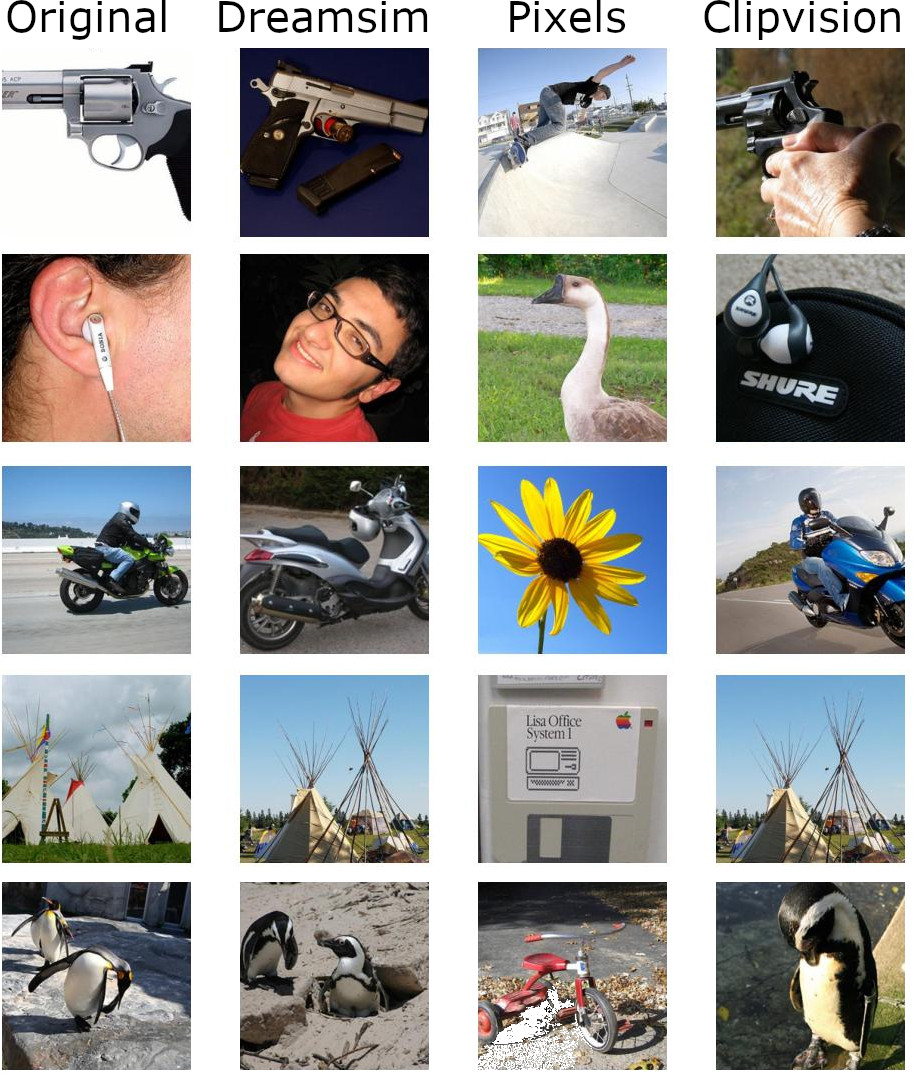
\includegraphics[width=0.6\textwidth]{plots/dropout_similarity_plot.JPEG}
  \caption[Qualitative results of diversity based subsampling]{Qualitative results of diversity based subsampling. In the left column, a random selection of 5 images from the original training dataset is shown. In the following columns, the most similar image to that original image in subsample based on the respective feature space (dreamsim, pixels and CLIP Vision) is shown.}\label{fig:dropout_similarity_plot}
\end{figure}

\rTwo{To measure if the subselections have properly increased the diversity in their respective subspaces, the previously described Average Min Distance is calculated for all three feature spaces }and is shown in Figure~\ref{fig:dropout_avg_min_distance}. For each subspace, 30 different samples were taken and the Average Min Distance was calculated for each sample. The figure shows that in each feature space, the subsample created using the corresponding feature space has the lowest Average Min Distance. The result is most ambiguous for the Average Min Distance in the pixel feature space, but again the subsample created using the pixel space has the lowest Average Min Distance. The Average Min Distance for dreamsim and CLIP Vision are always comparatively close, which makes sense since dreamsim is partly based on CLIP Vision~\cite{fuDreamSimLearningNew2023}. In summary, the qualitative and quantitative review showed that the diversity-based subsampling method is successful in increasing the diversity in the respective subspace. For each feature space, the subsample with the lowest Average Min Distance in the validation (i.e.\ best representing the entire feature space) is used for further analysis.

\begin{figure}[ht]
  \centering
  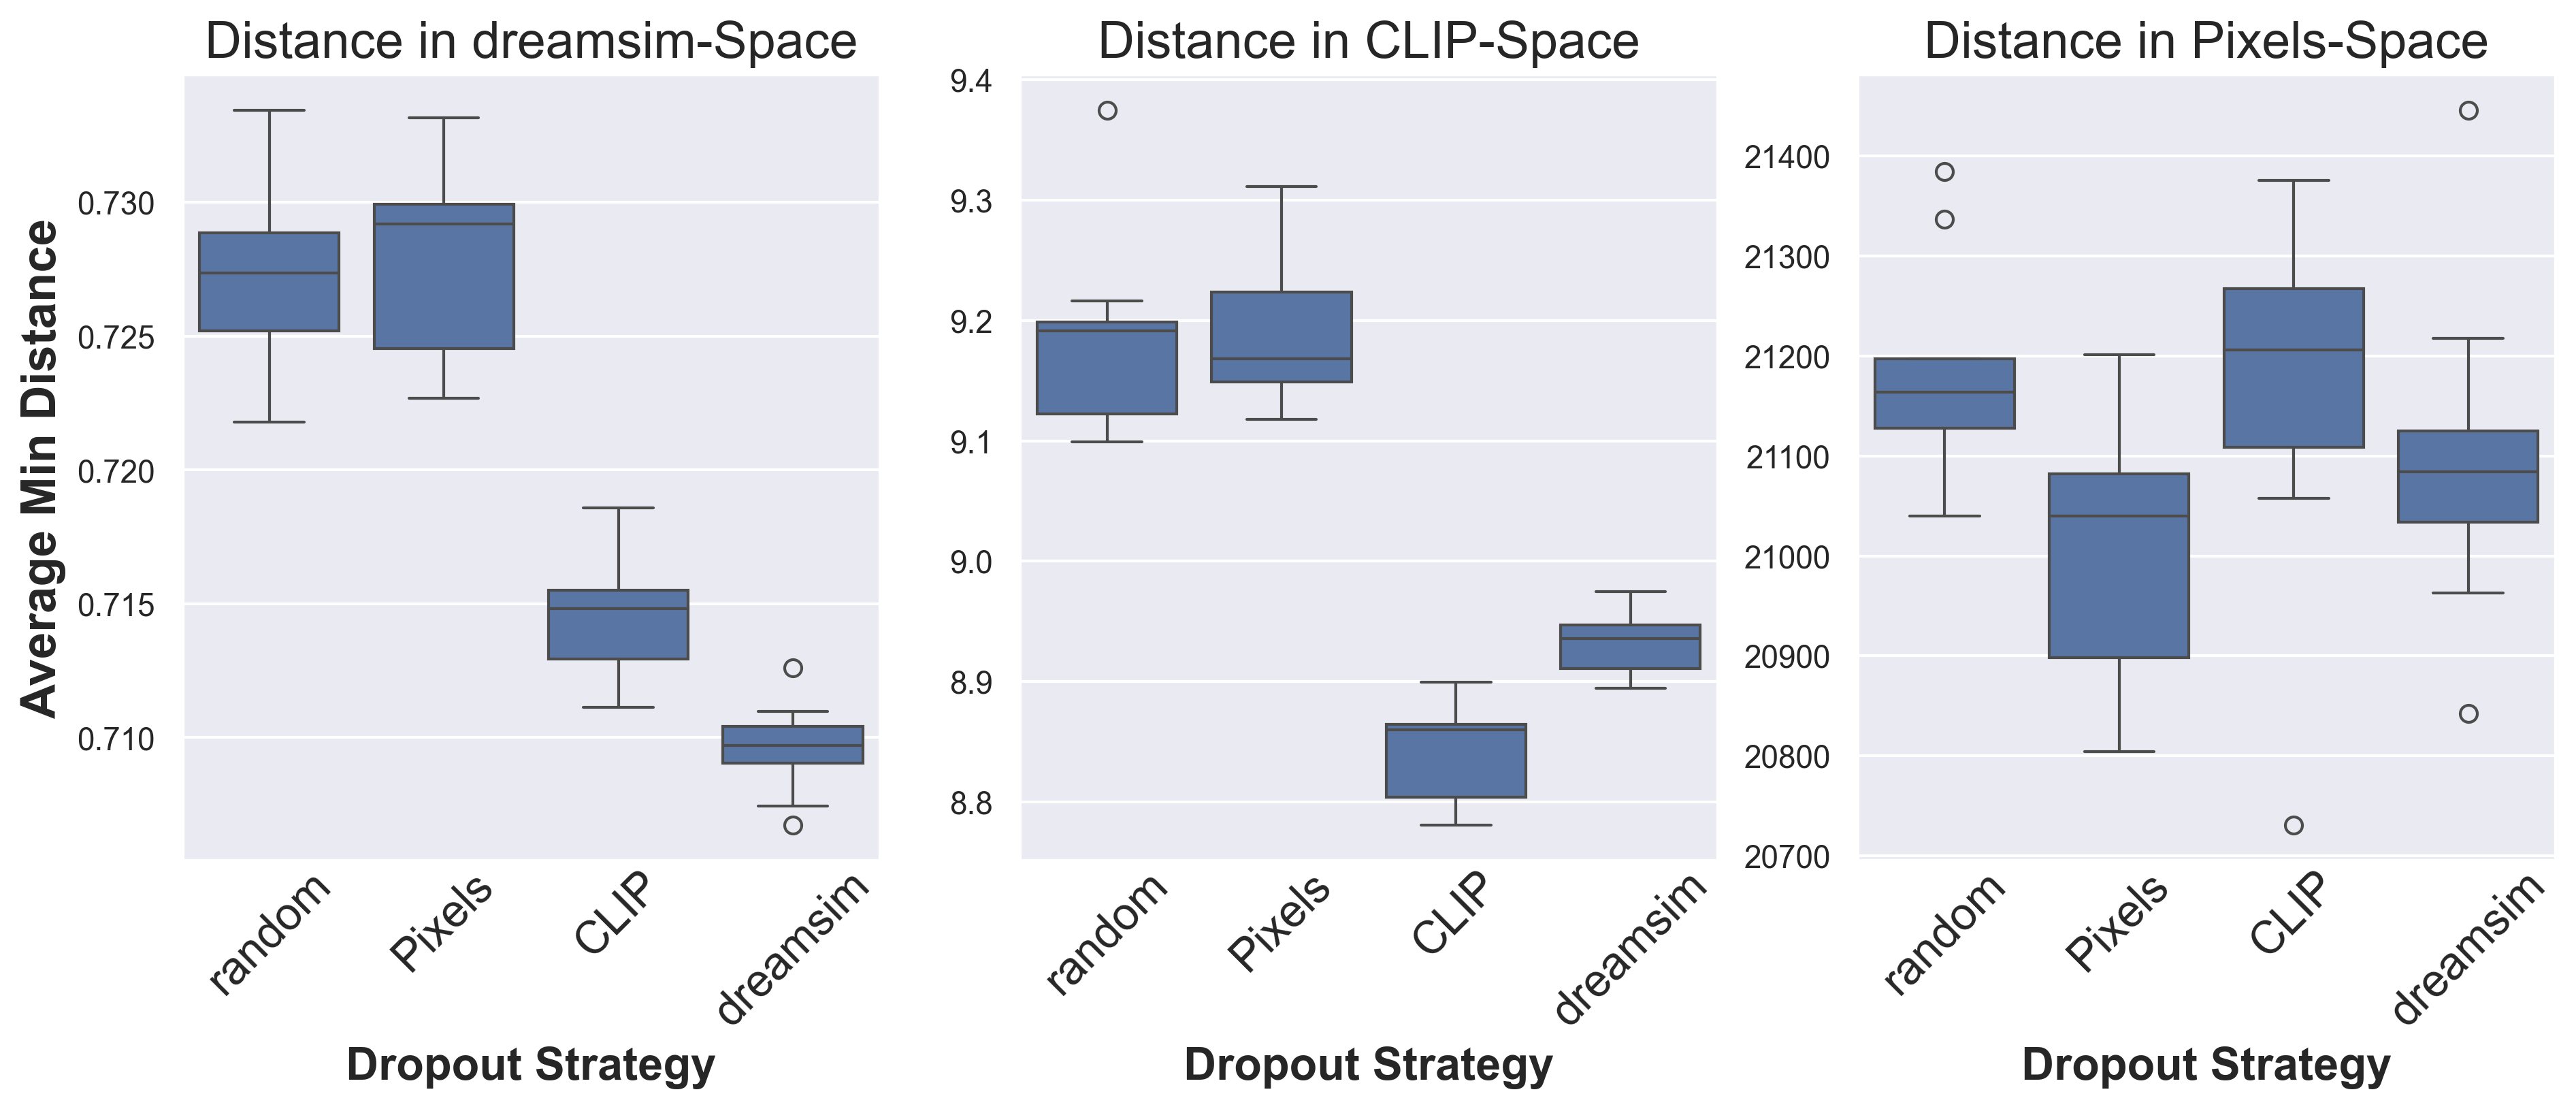
\includegraphics[width=1\textwidth]{plots/dropout_avg_min_distance.png}
  \caption[Average Min Distance with different dropout strategies]{Average Min Distance of multiple drawn subsamples. For each of the four dropout strategies (random and the three different features spaces), 30 samples with 25\% of the original dataset size were drawn. The Average Min Distance was computed within the three feature spaces and it's distribution across the 30 samples is plotted.}\label{fig:dropout_avg_min_distance}
\end{figure}


\subsubsection{Translator performance}
The performance of the three trained \rOne{translators} of the Brain-Diffuser and the iCNN algorithm is shown in Figure~\ref{fig:dropout_eval_translator_test} for the natural test images. The results are shown for all four different dropout strategies (random subsample and samples based on the three feature spaces). The performance of all subsamples is above the random probability of 0.5. However, for the three \rOne{translators} of the Brain-Diffuser, there are no discernible differences in performance between the different dropout strategies. Only the iCNN \rOne{translator} shows that performance can be slightly improved with a targeted diversity-based subsampling strategy. \rTwo{In} this case too, there is no significant difference between the three feature spaces. The artificial shapes in Figure~\ref{fig:dropout_eval_translator_art} show that the two CLIP translators are not able to predict the features significantly beyond random probability. This is independent of the subsampling space. The performance of the VDVAE translator is slightly better, with all subsamples tending to be better than the random probability. In particular, the performance of the low-level pixel feature space seems to have a slight advantage over the other subsampling strategies. For the iCNN translator, on the other hand, the effect of the natural test images seems to have been reversed; for the Pixel and dreamsim feature spaces, the performance even looks slightly worse than with random subsampling. Within the CLIP Vision feature space, the variance between the subjects is really high, thus the results cannot easily be interpreted.

% Now the Eval Results
% 7.1 Eval decoder test
\begin{figure}[ht]
  \centering
  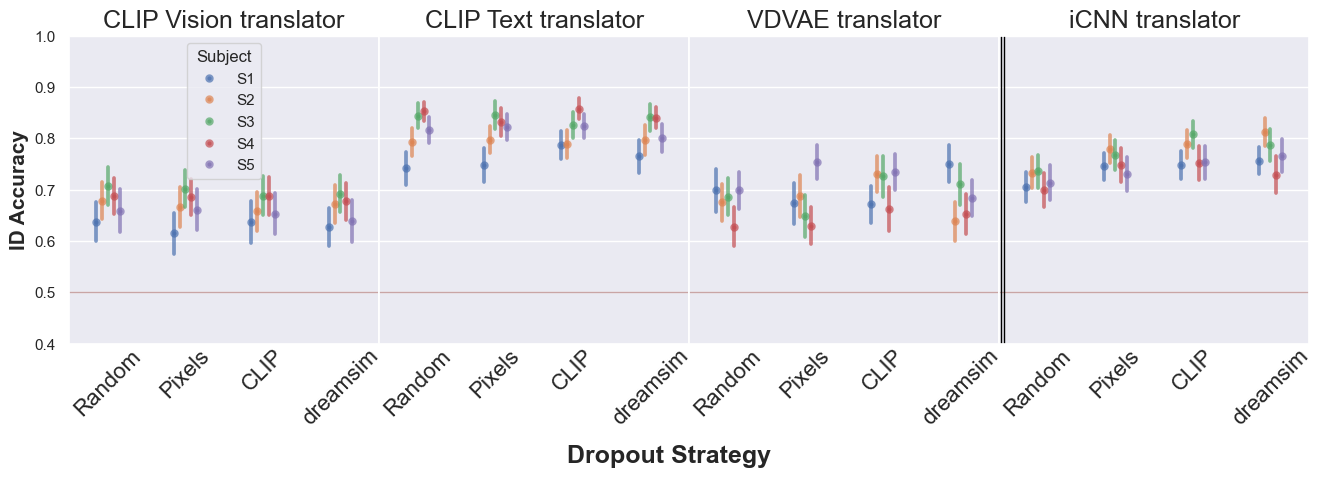
\includegraphics[width=1\textwidth]{plots/dropout_eval_translator_test.png}
  \caption[Experiment 1: Translator performance for natural test images]{\rOne{Translator} performance (0.25 data fraction) for natural test images. The identification accuracy for all four translators (three from Brain-Diffuser and one from iCNN) are displayed for the subsamples computed with the four dropout strategies. The data is shown for each subject and the error bars are computed as the standard errors across all test samples.}\label{fig:dropout_eval_translator_test}
\end{figure}


\begin{figure}[ht]
  \centering
  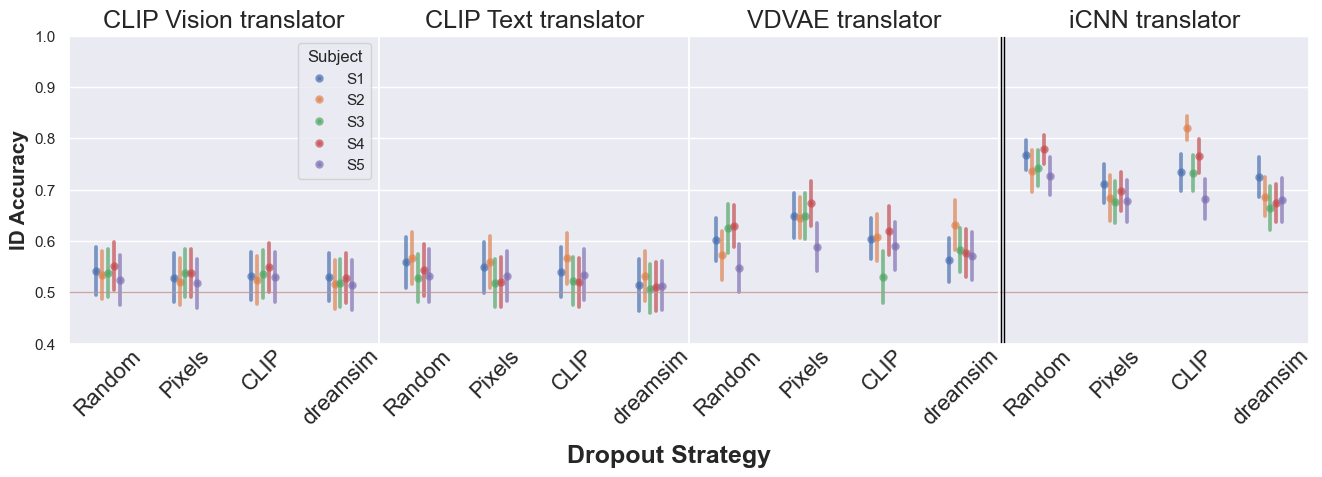
\includegraphics[width=1\textwidth]{plots/dropout_eval_translator_art.png}
  \caption[Experiment 1: Translator performance for artificial shapes]{\rOne{Translator} performance (0.25 data fraction) for artificial shapes. The identification accuracy for all four translators (three from Brain-Diffuser and one from iCNN) are displayed for the subsamples computed with the four dropout strategies. The data is shown for each subject and the error bars are computed as the standard errors across all test samples.}\label{fig:dropout_eval_translator_art}
\end{figure}


\subsubsection{Reconstruction performance}

\begin{figure}[ht]
  \centering
  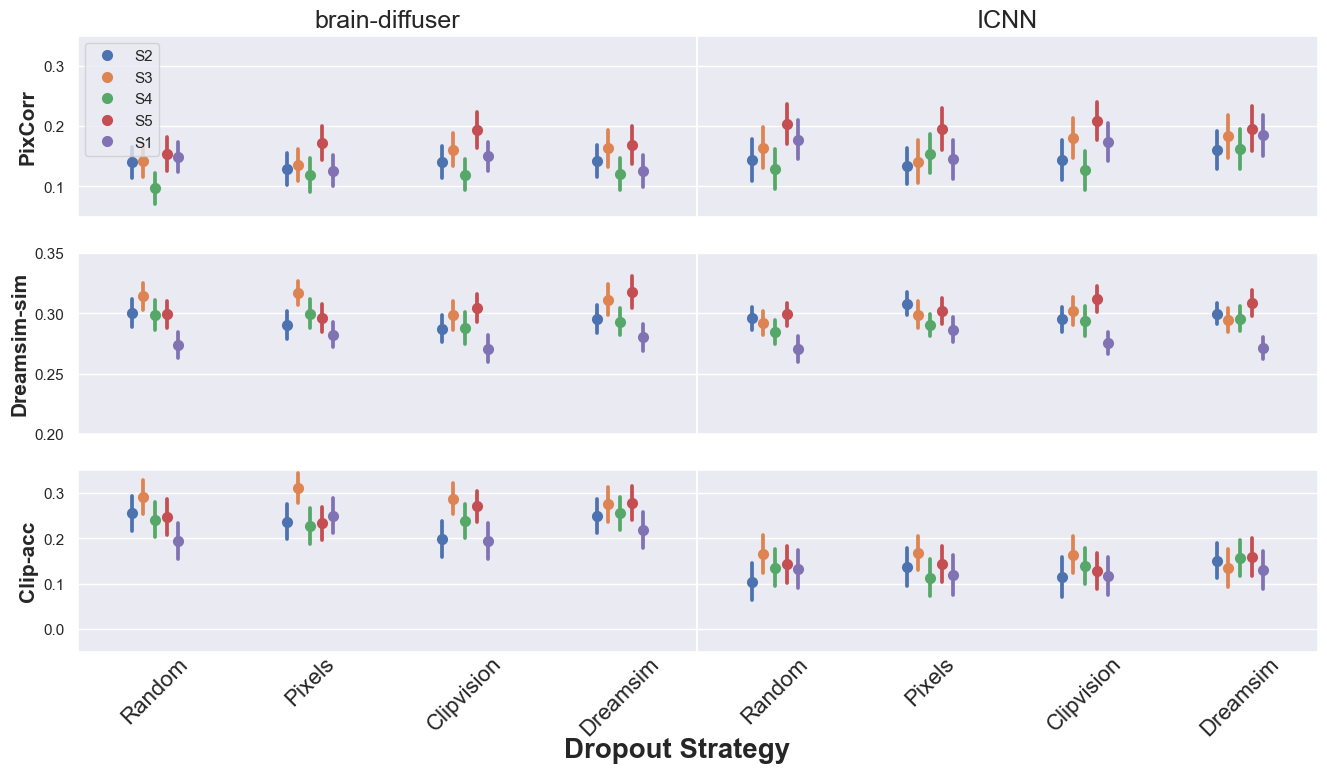
\includegraphics[width=1\textwidth]{plots/dropout_eval_reconstruction_test.png}
  \caption[Experiment 1: Reconstruction performance for natural test images]{Reconstruction Performance (0.25 data fraction) for natural test images. For each of the five subjects, the three reconstruction criteria (PixelCorrelation, dreamsim and CLIP-accuracy) are displayed for both the Brain-Diffuser and iCNN algorithm using the subsamples computed with the four dropout strategies. The errorbars are computed as the standard error across all the test samples.}\label{fig:dropout_eval_reconstruction_test}
\end{figure}

The quantitative results of the reconstructions using the four different subsamples are shown in Figure~\ref{fig:dropout_eval_reconstruction_test} for the natural test images. The three previously described criteria of PixelCorrelation, dreamsim-similarity and CLIP-accuracy are displayed for the Brain-Diffuser and iCNN algorithms respectively. There is no discernible difference between the random subselection and the three diversity-based subsamples for the Brain-Diffuser in any of the three metrics. The results are similar for the iCNN.\@ Although the translator performance was improved beforehand, these effects seem to have only a minor impact on the reconstruction performance. Only with the help of the dreamsim-similarity metric is there a slight increase in performance across all three feature spaces in contrast to the random baseline. There are again no differences between the feature spaces. Also for the artificial shapes in Figure~\ref{fig:dropout_eval_reconstruction_art}, the differences in reconstruction performance between the different feature spaces are small. For the Brain-Diffuser it looks as if the pixel correlation with a dropout is slightly increased in the pixel subspace compared to the baseline. There are no visible differences in the other metrics. In the iCNN, the dreamsim similarity appears slightly reduced in Pixels subspace and CLIP Vision subspace compared to the baseline. There are no visible differences in the dreamsim subspace.

\begin{figure}[ht]
  \centering
  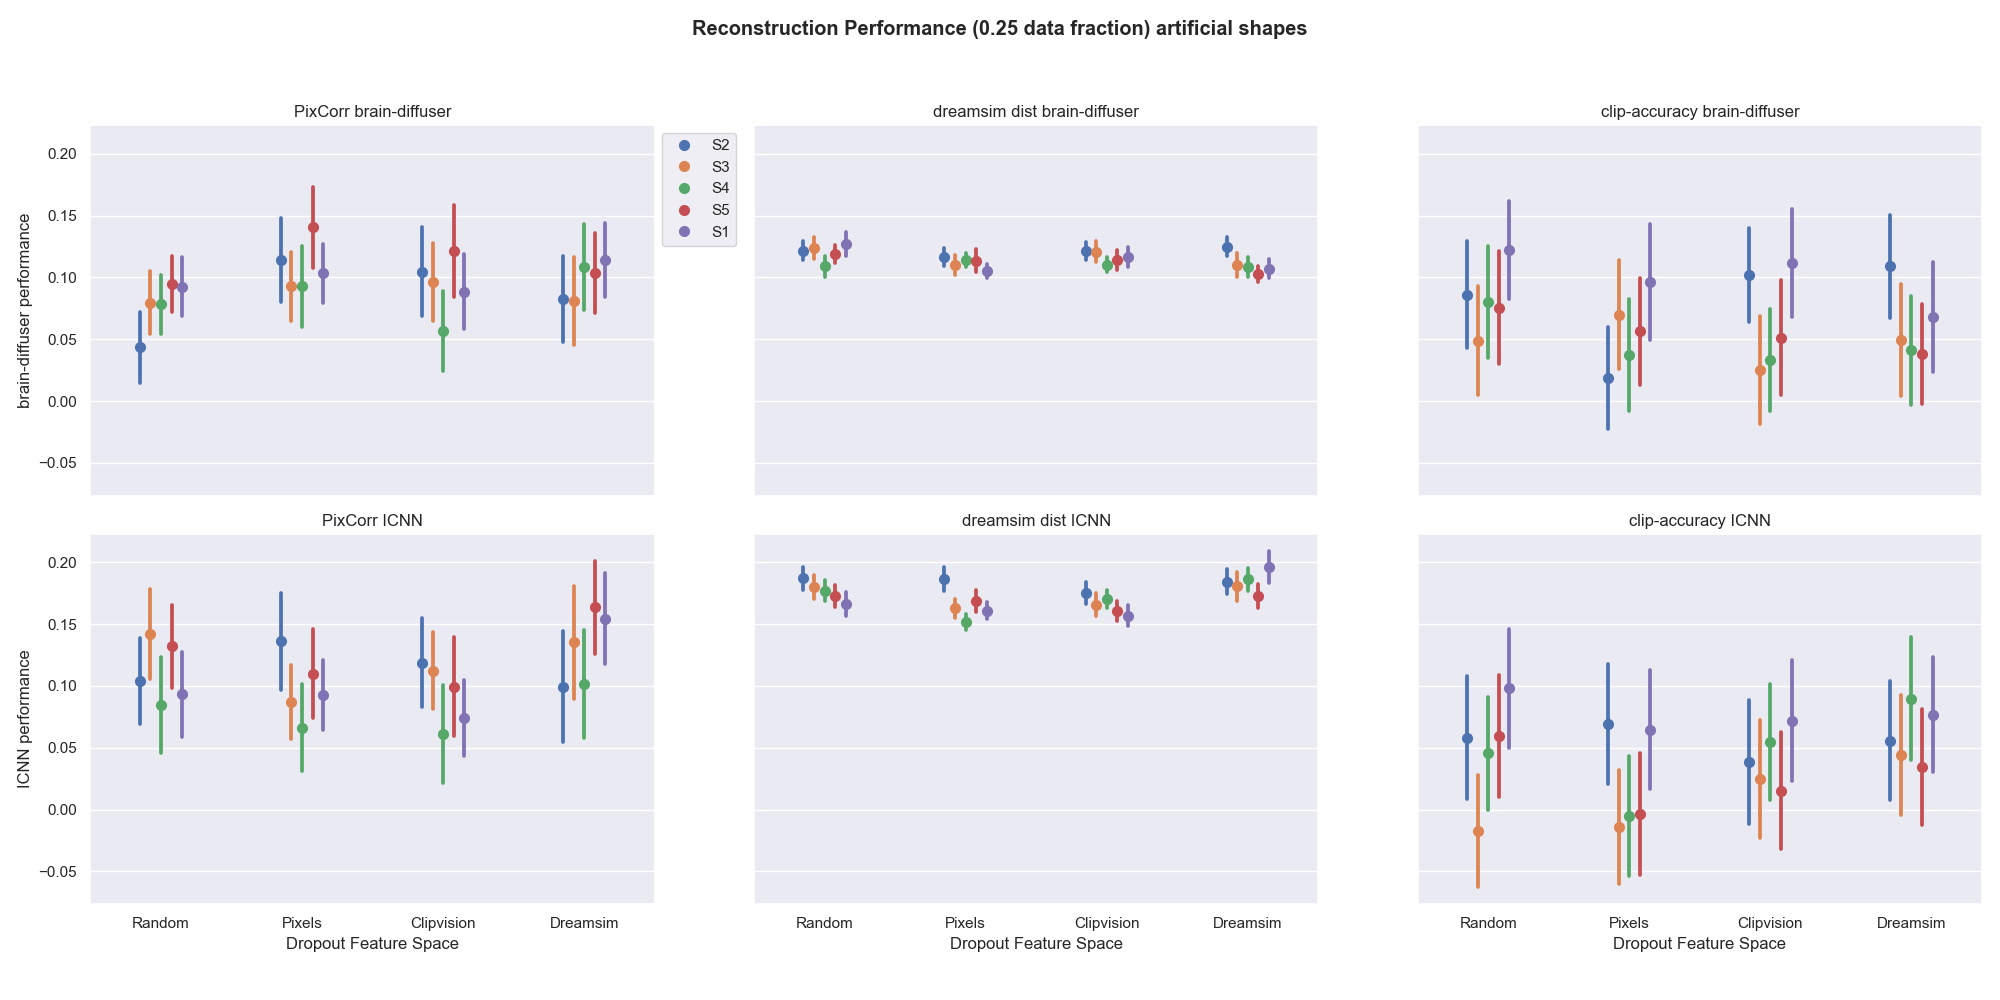
\includegraphics[width=1\textwidth]{plots/dropout_eval_reconstruction_art.png}
  \caption[Experiment 1: Reconstruction performance for artificial shapes]{Reconstruction Performance (0.25 data fraction) for artificial shapes. For each of the five subjects, the three reconstruction criteria (PixelCorrelation, dreamsim and CLIP-accuracy) are displayed for both the Brain-Diffuser and iCNN algorithm using the subsamples computed with the four dropout strategies. The errorbars are computed as the standard error across all the test samples.}\label{fig:dropout_eval_reconstruction_art}
\end{figure}


\begin{figure}[ht]
  \centering
  \includegraphics[width=1\textwidth]{plots/dropout_qual_eval_icnn_test.JPEG}
  \caption[Experiment 1: Reconstructed images for iCNN on natural test images]{Qualitative Results for different dropout strategies with the iCNN on natural test images. The top row depicts the ground truth image. Each following row depicts the reconstruction where the translator was trained using the dropout strategy defined on the left side.}\label{fig:dropout_qual_eval_icnn_test}
\end{figure}

As the quantitative results of the reconstruction performance suggest, a qualitative assessment of the differences in the reconstruction is difficult. The iCNN results for the natural test images are shown in Figure~\ref{fig:dropout_qual_eval_icnn_test}. Differences in the quality of the reconstruction are difficult to determine; although it is clear that at least some reconstruction quality can be achieved in all conditions, the slight improvement of the feature spaces in contrast to the random baseline  seen in the quantitative results is not immediately apparent in the actual images. Likewise, for the artificial shapes in Figure~\ref{fig:dropout_qual_eval_icnn_art}, the slight degradation in the feature space results compared to the random sample is not directly apparent from the qualitative results. The quantitative results for the Brain-Diffuser were even more ambiguous, so no major differences can be seen in the qualitative analysis of the images. The reconstructed images for the Brain-Diffuser can be found in the appendix (Figure~\ref{fig:dropout_qual_eval_bd_test} for the natural test images and Figure~\ref{fig:dropout_qual_eval_bd_art} for the artificial shapes).


\begin{figure}[ht]
  \centering
  \includegraphics[width=1\textwidth]{plots/dropout_qual_eval_icnn_art.JPEG}
  \caption[Experiment 1: Reconstructed images for iCNN on artificial shapes]{Qualitative Results for different dropout strategies with the iCNN on artificial shapes. The top row depicts the ground truth image. Each following row depicts the reconstruction where the translator was trained using the dropout strategy defined on the left side.}\label{fig:dropout_qual_eval_icnn_art}
\end{figure}

\subsection{Discussion}
  
\rTwo{Our initial hypotheses were only partially confirmed, revealing more complex relationships between data diversity and reconstruction performance than anticipated. We hypothesized that low-level feature diversity would improve performance on artificial shapes, high-level diversity would benefit natural images, and mid-level diversity would provide the best overall performance. The results revealed several unexpected patterns that provide new insights into how different aspects of visual information are processed and reconstructed from brain activity.} For the Brain-Diffuser, there were generally few differences between the different subsamples. Only for the artificial shapes could the translator performance and also the pixel correlation of the reconstruction be increased by low-level subsampling. This is consistent with the hypothesis that low-level subsampling improves low-level reconstruction. However, as this effect can only be measured with the pixel correlation, it should be treated with caution and could only have occurred by chance. With the iCNN the results were somewhat clearer. In the case of the natural test images, the \rOne{translator} could be improved by any type of subsampling, and the subsequent reconstructions could also be improved (measured with dreamsim). Interestingly, this effect is exactly the opposite for the artificial shapes. Here, diversity-based subsampling even seems to be disadvantageous compared to random subsampling: both the \rOne{translator} and the reconstruction performance decrease compared to the baseline. 

\subsubsection{Exploring the influence of monotone training data}
In the following, we will further investigate why the performance of the artificial shapes is presumably reduced by diversity-based subsampling. A closer look at the training images reveals that there are some images that show individual central objects with a monotonous (usually white) background. It could be that these are similar in concept to the artificial shapes. In this sense, the artificial shapes would not really be out-of-distribution samples, because a monotone background of the training images is not really natural either. It is investigated whether these images have a significant influence on the reconstruction. In order to test this, a new, reduced training data set is created, which mainly contains these images. A simple algorithm is used to identify these images in the training dataset automatically: The colour values for each pixel in all images are counted, and then the images are sorted according to how often the most frequent pixel occurs in each image (so an image with a white background would have the colour white as most frequent color, which occurs extremely often). In figure~\ref{fig:dropout_discussion_monohetero_qual}, the 5 most monotonous images found by the algorithm (i.e.\ those where the most frequent colour occurs very often) are compared with the 5 most heterogeneous images (i.e.\ those where the colours are more evenly distributed). As can be seen, the subdivision of the images using this algorithm worked well. In the following, \rOne{translators} consisting of 0.25 (i.e. 300 images) of the training data for the most homogeneous and heterogeneous as defined by the algorithm explained above set are trained again.


\begin{figure}[ht]
  \centering
  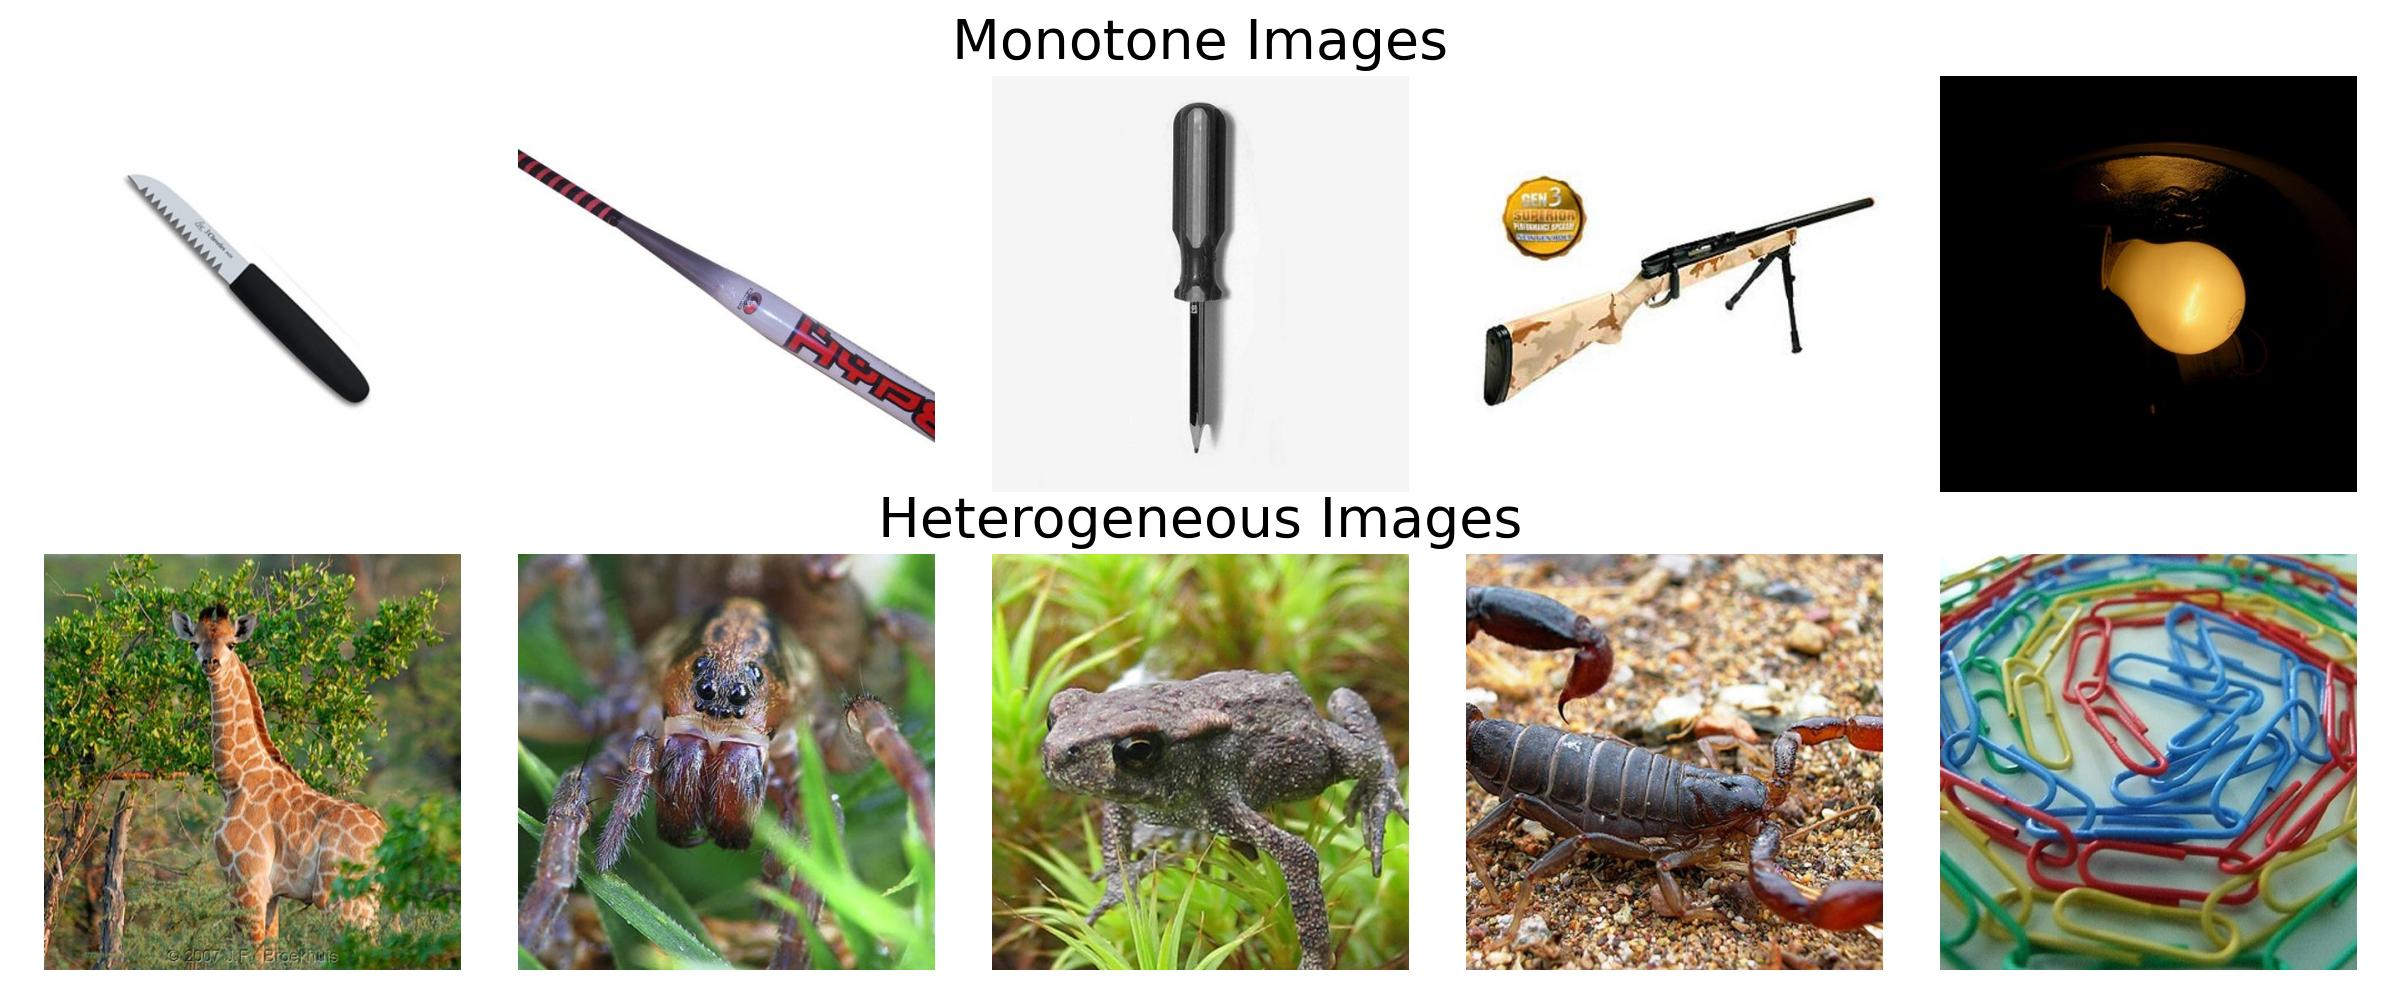
\includegraphics[width=1\textwidth]{plots/dropout_discussion_monohetero_qual.jpeg}
  \caption[Monotone and heterogeneous samples in the training dataset]{Comparison of monotone and heterogeneous training images (the five most monotone and heterogeneous samples are displayed).}\label{fig:dropout_discussion_monohetero_qual}
\end{figure}

\begin{figure}[ht]
  \centering
  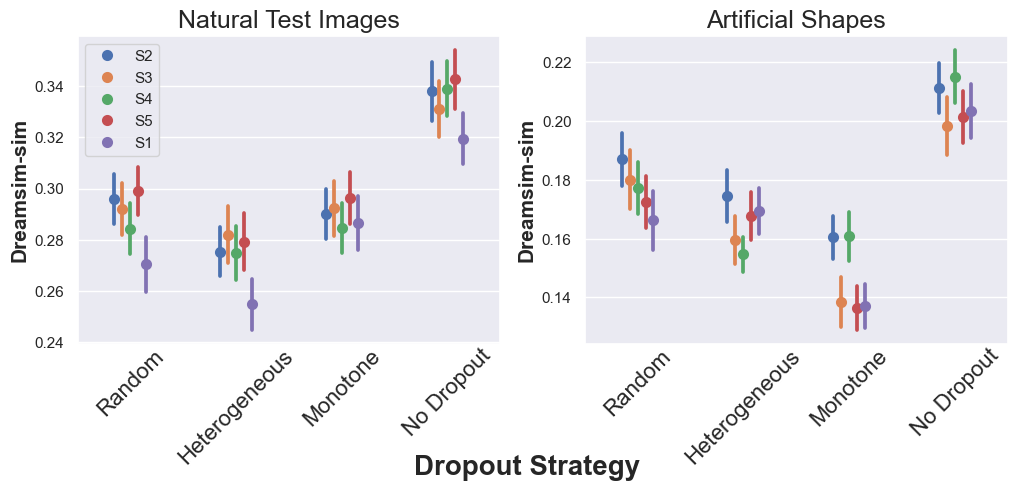
\includegraphics[width=1\textwidth]{plots/dropout_discussion_reconstruction_icnn.png}
  \caption[iCNN reconstruction performance monotone vs.\ heterogeneous training sample]{iCNN reconstruction results for monotone vs.\ heterogeneous training images. The dreamsim reconstruction metric is displayed for all five participants depending on the dropout strategy. The results for both the natural test images and artificial chapes are displayed. The error bars are computed as the standard error across all test samples.}\label{fig:dropout_discussion_reconstruction_icnn}
\end{figure}

The quantitative results of the reconstructions with the monotonous and heterogeneous subsample training datasets are shown in Figure~\ref{fig:dropout_discussion_reconstruction_icnn} for both the natural test images and the artificial shapes. The random dropout performs better than both monotonous and heterogeneous subsampling. Contrary to expectation, monotonous subsampling actually performs worse than heterogeneous subsampling with artificial shapes. \rTwo{The} results for the Brain-Diffuser (displayed in Figure~\ref{fig:dropout_discussion_reconstruction_bd}) are quite different. As expected, random subsampling performs best for natural test images. For the artificial shapes, however, there is a clear effect: monotonous subsampling leads to significantly better performance than heterogeneous subsampling. It is even on par with the performance that can be expected, if there is no dropout at all (all training images are used). This effect is also best illustrated by the qualitative reconstructions for the natural test images in Figure~\ref{fig:dropout_discussion_test} (the qualitative results for the artificial shapes are shown in Figure~\ref{fig:dropout_discussion_art} in the appendix): for each image reconstructed with the Brain-Diffuser, a monochrome background can be seen in the monotonous condition. In contrast, all backgrounds show multiple details when the heterogeneous training data is used. This also shows why the results of the iCNN for the artificial shapes are not necessarily improved by using monotonous training: the reconstructions with the iCNN have a comparatively neutral background when both monotonous and heterogeneous training data are used. All results for the four different translators for monotonous vs.\ heterogeneous training data are shown in the appendix in figures~\ref{fig:dropout_discussion_translator_id_acc_cliptext},~\ref{fig:dropout_discussion_translator_id_acc_clipvision},~\ref{fig:dropout_discussion_translator_id_acc_vdvae},~\ref{fig:dropout_discussion_translator_id_acc_icnn}. 

The insights that can be gained from this additional investigation using monotonous and heterogeneous training data subsets are twofold. On the one hand, the Brain-Diffuser can be strongly conditioned to reconstruct single objects with monotonous backgrounds, so that the performance for the artificial images can be greatly improved by the background of the images alone. There is even no quantitative performance increase if all training images would be used instead of only the ones with monotone background. On the other hand, it can be seen that the iCNN generally seems to produce images with neutral backgrounds and a central object in the middle (this can also be checked with the other qualitative results in this experiment). It therefore seems that the iCNN has a bias towards this type of image, where single central objects are displayed on a neutral background, regardless of the nature of the training data. The reason for this bias in the iCNN might be the pre-training of the model on the ImageNet~\cite{dengImageNetLargescaleHierarchical2009} dataset --- the images also mostly feature a prominent object in the middle. Another reason for this phenomenon could lie in the way the visual attention works. It has been shown that visual attention strongly modulates the translation of brain-activity~\cite{horikawaAttentionModulatesNeural2022}. Since the participants probably focused on the prominent central aspects of the images when their brain activity was recorded, only these central aspects of the training images might have caught the attention of the subjects, thus having a stronger representation in the brain activity~\cite{wolfeVisualAttention2000}. 

\begin{figure}[ht]
  \centering
  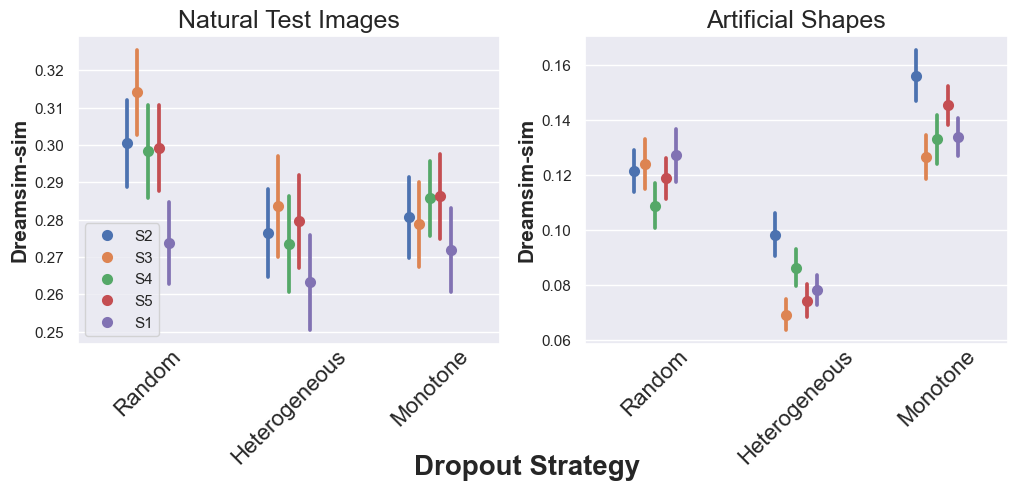
\includegraphics[width=1\textwidth]{plots/dropout_discussion_reconstruction_bd.png}
  \caption[Brain-Diffuser reconstruction performance monotone vs.\ heterogeneous training sample]{Brain-Diffuser reconstruction results for monotone vs.\ heterogeneous training images. The dreamsim reconstruction metric is displayed for all five participants depending on the dropout strategy. The results for both the natural test images and artificial chapes are displayed. The error bars are computed as the standard error across all test samples.}\label{fig:dropout_discussion_reconstruction_bd}
\end{figure}

\begin{figure}[ht]
  \centering
  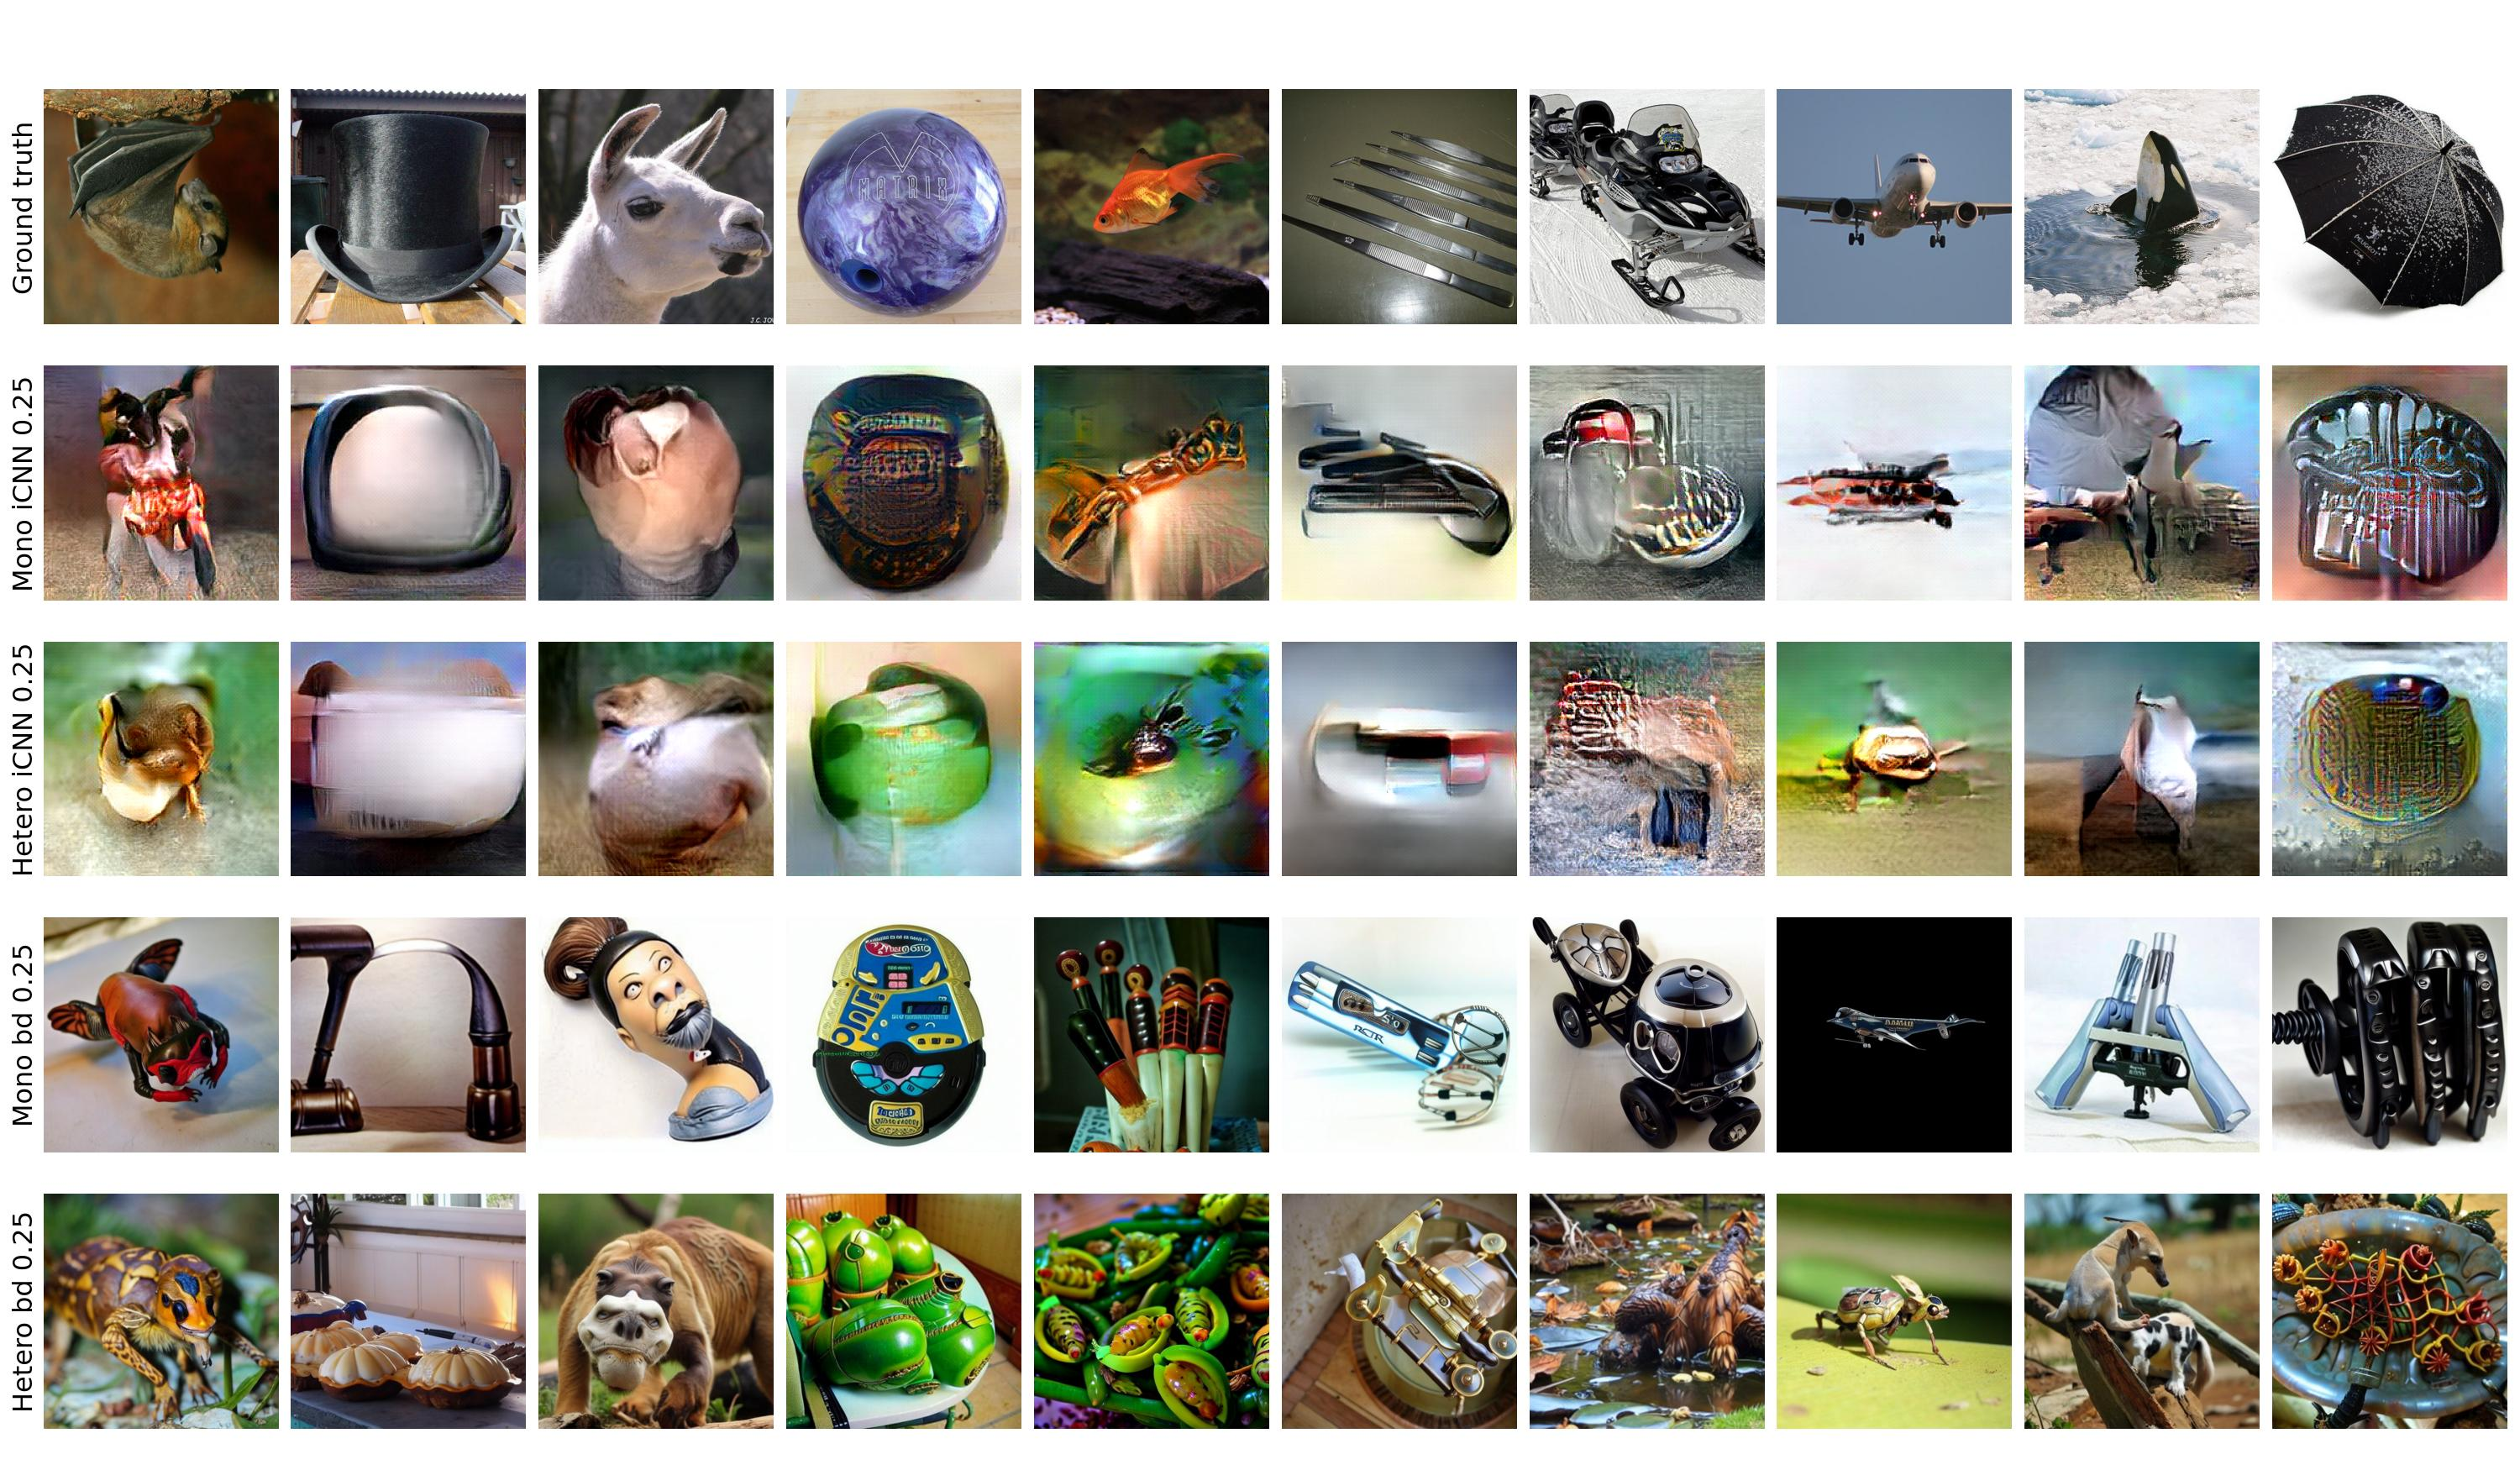
\includegraphics[width=1\textwidth]{plots/dropout_discussion_test.JPEG}
  \caption[Reconstructed images monotone vs.\ heterogeneous training samples]{Qualitative Results for monotone vs.\ heterogeneous training images on natural test images. The top row depicts the ground truth image. Each following row depicts the reconstruction where the translator was trained using the dropout strategy and reconstruction algori defined on the left side (Note: bd stands for Brain-Diffuser).}\label{fig:dropout_discussion_test}
\end{figure}

\subsubsection{Future directions}

The results of the dropout experiment showed that the diversity of the training data set can have a significant influence on the \rOne{translation} of brain activity and the reconstruction of images. However, the exact direction and nature of the influence on the  reconstructions is still unclear. The results of this study were inconclusive in this respect. Further research is needed on the influence of the diversity of training images on brain \rOne{activity translation}. To this end, further different types of dropout could be used. For example, it would be possible to use dropout based on the actual semantic categories (e.g.\ using the stimulus code), so that the results do not depend on the UMAP embedding and random initial conditions during clustering. Furthermore, a more sophisticated algorithm could be used to separate the monotonous from the heterogeneous images that would also include semantic information. 

One limitation of the study is that subsampling is only possible top-down. This means that a large data set is required, which is first reduced. Ideally, there would be a way to evaluate the quality of an existing subsample iteratively from a bottom-up perspective  to determine what an image should look like that needs to be added to the dataset to improve the performance. One possibility could be an active learning approach~\cite{senerActiveLearningConvolutional2018, guoDeepCoreComprehensiveLibrary2022}, which could be used during training to always look for the next image that would improve the performance. Ultimately, the aim of this research is to investigate how the nature of a dataset needs to be in order to optimise reconstruction performance. For instance an approach like the one of Couch et al.~\cite{couchSizeClassBalance2024} could be used, that measures the dataset quality/diversity in a single metric. These results could then be used to create optimised training data sets that would be shown to subjects in future MRI studies. This optimised training data set does not necessarily have to consist of a sub-sample of natural images. Dataset distillation~\cite{wangDatasetDistillation2018,yuDatasetDistillationComprehensive2024} could be used to create an artificial training dataset that is optimised to improve the \rOne{translation}, allowing better generalisation to all possible test images. Further research is needed to determine how such an artificial training dataset might look like and whether, for example, it is necessary to show subjects natural training images at all or if it might be better to only show abstract, generated images. 

In summary, this experiment showed that diversity-based subsampling has an impact on reconstruction performance, but that this impact needs further investigation in terms of direction and exact magnitude. In particular, the Brain-Diffuser algorithm performed very poorly with the artificial shapes, and its \rOne{translator} performance improved only marginally even with a larger amount of training data (see the random dropout results). The following experiments therefore look for ways to improve the performance of the Brain-Diffuser, especially with artificial shapes.
